% easychair.tex,v 3.1 2011/12/30
%
% Select appropriate paper format in your document class as
% instructed by your conference organizers. Only withtimes
% and notimes can be used in proceedings created by EasyChair
%
% The available formats are 'letterpaper' and 'a4paper' with
% the former being the default if omitted as in the example
% below.
%
\documentclass[procedia]{easychair}
%\documentclass[debug]{easychair}
%\documentclass[verbose]{easychair}
%\documentclass[notimes]{easychair}
%\documentclass[withtimes]{easychair}
%\documentclass[a4paper]{easychair}
%\documentclass[letterpaper]{easychair}

% This provides the \BibTeX macro
\usepackage{doc}
\usepackage{makeidx}

% TODO please include it
\usepackage{subfig}
\usepackage{graphicx}

% In order to save space or manage large tables or figures in a
% landcape-like text, you can use the rotating and pdflscape
% packages. Uncomment the desired from the below.
%
% \usepackage{rotating}
% \usepackage{pdflscape}

% If you plan on including some algorithm specification, we recommend
% the below package. Read more details on the custom options of the
% package documentation.
%
% \usepackage{algorithm2e}

% Some of our commands for this guide.
%
\newcommand{\easychair}{\textsf{easychair}}
\newcommand{\miktex}{MiK{\TeX}}
\newcommand{\texniccenter}{{\TeX}nicCenter}
\newcommand{\makefile}{\texttt{Makefile}}
\newcommand{\latexeditor}{LEd}

\def\procediaConference{Youth Science Conference 2017}

%\makeindex

%% Front Matter
%%
% Regular title as in the article class.
%
\title{Absolute humidity anomalies and the influenza onsets in Russia: a computational study}

% \titlerunning{} has to be set to either the main title or its shorter
% version for the running heads. When processed by
% EasyChair, this command is mandatory: a document without \titlerunning
% will be rejected by EasyChair

\titlerunning{Absolute humidity anomalies and the influenza onsets in Russia\ldots}

% Authors are joined by \and. Their affiliations are given by \inst, which indexes into the list
% defined using \institute
%
\author{
    Nikita E. Seleznev\inst{1}
\and
    Vasiliy N. Leonenko\inst{2}
}

% Institutes for affiliations are also joined by \and,
\institute{
  ITMO University,
  Saint-Petersburg, Russia\\
  \email{ne.seleznev@gmail.com}
\and
   ITMO University,
   Saint-Petersburg, Russia\\
   \email{vnleonenko@yandex.ru}\\
 }
%  \authorrunning{} has to be set for the shorter version of the authors' names;
% otherwise a warning will be rendered in the running heads. When processed by
% EasyChair, this command is mandatory: a document without \authorrunning
% will be rejected by EasyChair

\authorrunning{Seleznev, Leonenko}

\begin{document}

\maketitle

\keywords{data analysis, mathematical epidemiology, acute respiratory infection, absolute humidity, seasonal influenza, Python}

\begin{abstract}
In the current work we use a computational approach to analyze the association between the anomalous drops of absolute humidity and the subsequent onset of influenza epidemics in Russia. The correlation between these two factors is searched relying on the data of acute respiratory infection incidence in Saint Petersburg, Moscow and Novosibirsk. The analysis results, along with the output from the same analysis for Ile-de-France region (Paris and its suburbs), were compared with those achieved by Dr. Jeffrey Shaman and his co-authors for the US states. We show that although the analysis results for Ile-de-France are in agreement with the conclusions of Dr. Shaman, it does not hold true for the case of Russia, where the relation between the low levels of absolute humidity and the influenza onset is proved to be statistically insignificant.
\end{abstract}

%\setcounter{tocdepth}{2}
%{\small
%\tableofcontents}

%\section{To mention}
%
%Processing in EasyChair - number of pages.
%
%Examples of how EasyChair processes papers. Caveats (replacement of EC
%class, errors).


%------------------------------------------------------------------------------
\section{Introduction}
\label{sect:introduction}

Influenza (or, shortly, flu) is one of the most common human infectious diseases. Being the most virulent among more than two hundred known seasonal acute respiratory infections (ARI), it causes repetitive outbreaks resulting in high worker/school absenteeism and productivity losses. Also, if left without proper treatment, influenza leads to complications that may cause death of infected persons (the annual mortality rate is from 250 to 500 thousand individuals, according to WHO \cite{who_flu_facts}). 

To reduce the number of improperly treatment cases of influenza it is beneficial for the healthcare organs to be prepared to the incoming epidemic in advance.  Although the seasonality of influenza outbreaks is widely known, its mechanism still doesn't have satisfactory explanation. A lot of factors are named that may influence the moment of the outbreak onset and its dynamics other time, but the extent of influence of one or another factor on the outbreak parameters is still  arguable. Nevertheless, most of the researchers have come to terms with the fact that the influence of absolute humidity (AH) levels should be taken into account \cite{tamerius2011global}, \cite{van2012role}. This statement was supported, among the other works, by the results of data analysis for the flu outbreaks in Russia \cite{romanyukha2011origin}, \cite{Leonenko2016}. The experiment performed by Shaman et al. demonstrated a hands-on biological justification showing that virus survival and transmission among guinea pigs increased monotonically with a decrease in AH \cite{shaman2009absolute}. In the subsequent paper the authors extend their previous findings to the human population level, showing that the onset of increased wintertime influenza-related mortality in the US is preceded by anomalously low absolute humidity levels \cite{shaman2010absolute}. As a result, the authors state that ``AH is a major (and likely predominant) determinant of influenza seasonality''. At the same time, they admitted that some of their experiment results contradicted this statement: particularly, the association between the AH drop and a subsequent influenza onset did not reach statistical significance in a big part of the Northwestern USA.

In this paper we aim to answer the question if the anomalous drops in AH may precede the influenza onsets in Russian Federation using the long-term ARI weekly incidence data in three cities (Moscow, Saint Petersburg and Novosibirsk) from 1986 to 2015. For this sake we adapt the idea of Shaman et al. to use it for our data at hand, implement the corresponding computational algorithm and perform the data analysis. The experiment results contribute to understanding whether the anomalous absolute humidity before the flu outbreaks may be found in Russian settings as well as in the USA and, thus, whether this phenomenon could be used to increase the quality of by far not-so-accurate model predictions obtained by the authors for flu dynamics in Russia \cite{leonenko2016mathbio}, \cite{Leon_Novo_Ong}. To perform the data analysis we have reconstructed the algorithm which aims at representing the average AH dynamics before and after influenza onsets and assesses the statistical significance of potentially abnormal AH dynamics. 

\section{Algorithm structure}

\subsection{Assessing $AH$ dynamics before and after the onset}

First of all, we need to form the dataset of $AH$ deviations before and after the onset. This is done according to the following sequence of operations:

\begin{itemize}
\item Form the array which contains all the days of influenza onsets corresponding to the selected year period and geographical locations (states, cities, countries) under consideration. These days may be available from external sources or be calculated by the algorithm itself based on some influenza outbreak criteria. Let $n$ be the overall number of onset days.

\item For $i \in \overline{1,n}$:
\begin{itemize}
\item Take a sample of $AH$ values corresponding to the continuous measurements during 6 weeks (42 days) before and 4 weeks (28 days) after the $i$-th onset for the corresponding year and a state (70 values in total).
\item Using the $AH$ sample, form a dataset $Z{^{(i)}}$ which contains corresponding values of $AH'$, local daily deviations of AH from its 31-year mean for each day (70 values in total).  
\end{itemize}

\item Let $Z^{(i)} = \{ Z^{(i)}(-42), Z^{(i)}(-41), \dots, Z^{(i)}(27)\}$, $i \in \overline{1,n}$, where $Z^{(i)}(0)$ corresponds to the value of $AH'$ in the day of influenza onset. Form the averaged sample $Z$: $Z(j) :=  \frac{\sum^{n}_{i=1} Z^{(i)}(j)}{n}$, $j \in \overline{-42,27}$. 
\end{itemize}

$Z$ is the average of $AH'$ values which we are going to investigate further to find anomalous drops (corresponding to extremely low values of $AH'$). The simplest way of doing it is to seek them visually on the $AH'$ graphs. However, since the visual comparison of graphs is highly subjective and thus error-prone, it seems reasonable to assess the significance of the observed abnormal drops with the help of statistical tests. 

\subsection{Statistical testing}
\label{sect:stats}
In order to determine statistical significance of an $AH'$ deviation from the level $AH' = 0$, a bootstrapping using a Monte Carlo sampling procedure was used similar to the one used in \cite{shaman2010absolute}. Our aim was to accept or deny for the each state the null hypothesis: samples of $AH'$ dynamics preceding the epidemic onset do not differ significantly from the randomly chosen arbitrary samples of $AH'$ dynamics throughout the year. 

To test this hypothesis two samples of $AH'$ are generated. One consists of the averaged values of $AH'$ throughout the wintertime seasons sampled randomly in time and space (it can be named ``arbitrary sample''), another one is comprised of the averaged $AH'$ prior to the influenza onset (``preonset sample''). The algorithm aimed at generating these samples is described below.

\paragraph{Arbitrary $AH'$ sample generation.}
For $i \in \overline{1,100000}$ do:
\begin{itemize}
	\item Let $X$ be an empty set. 
		Repeat $n$ times, where $n$ is a total onset events number for a given threshold:
	\begin{itemize}
		\item Choose randomly a year, a state and a day within the winter season (from October 1 to April 30).
		\item Take a sample of $AH'$ values corresponding to the continuous measurements during 4 weeks prior to the selected day for a chosen year and a state (28 $AH'$ values in total).
	\end{itemize}
	\item Find sample mean and add it to $X$. 
\end{itemize}
The resulting set $X$ is the arbitrary sample.

\paragraph{Preonset $AH'$ sample generation.}
Let $Y$ be an empty set, $n$ be the total number of registered influenza onsets in different states in different years. For $i \in \overline{1,n}$ do:
\begin{itemize}
	\item Take a sample of $AH'$ values corresponding to the continuous measurements during 4 weeks prior to the $i-th$ onset (for the corresponding year and a state).
	\item Find sample mean and add it to $Y$. 
\end{itemize}
The resulting set $Y$ is the preonset sample.

\paragraph{Hypothesis testing.}
To check if the samples $X$ and $Y$ have the same mean, we use Welch's t-test. This test, apart from the commonly used Student's t-test, does not require equal sample variance. Let null hypothesis be such that samples have identical means. The test measures whether the mean values of the samples differ significantly. In case if $p$-value$<0.05$ we reject the null hypothesis, i.e. we state that our preonset sample of $AH'$ significantly differs from the arbitrary sample. That will correspond to the case of anomalous $AH'$ drop. On the other hand, if $p$-value is large, then we cannot assume a statistically significant drop in $AH'$ prior to the epidemic onsets.


%------------------------------------------------------------------------------
\section{Anomalous AH drops analysis}

The algorithm described above was implemented as a set of procedures in Python 3.x programming language, using the libraries \texttt{numpy}, \texttt{matplotlib} and \texttt{scipy.stats}. Having created a tool of analysis, we applied it to datasets at hand to analyze $AH$ drops in various geographical settings.

\subsection{Influenza onsets in the USA} \label{sect:usa}

To ensure the correctness of our implementation of the algorithm, we decided to start with reproducing the graphs from \cite{shaman2010absolute} using the original data kindly provided by Dr. Shaman. Also we wanted to extend the original work by analyzing the AH' drops in separate US states.

\paragraph{Data.}

The $AH$ dataset we used contained daily absolute humidity ($AH$) in the US states from 1972 to 2002. Since the ready-made dataset on influenza onset dates was not available, those dates were assessed using the data on weekly pneumonia and influenza mortality ($P\&I$ mortality). The particular date was considered to be a date of influenza onset in the particular location (US state) if it belonged to wintertime period and the corresponding $P\&I$ mortality had been at or above a prescribed threshold level (e.g., 0.01 deaths/100,000 people/day) during the two preceding weeks. 

\paragraph{Reproducing the results for the USA as a whole.}

\begin{figure}
	\begin{center}
		\begin{tabular}{ccc}
			\subfloat[]{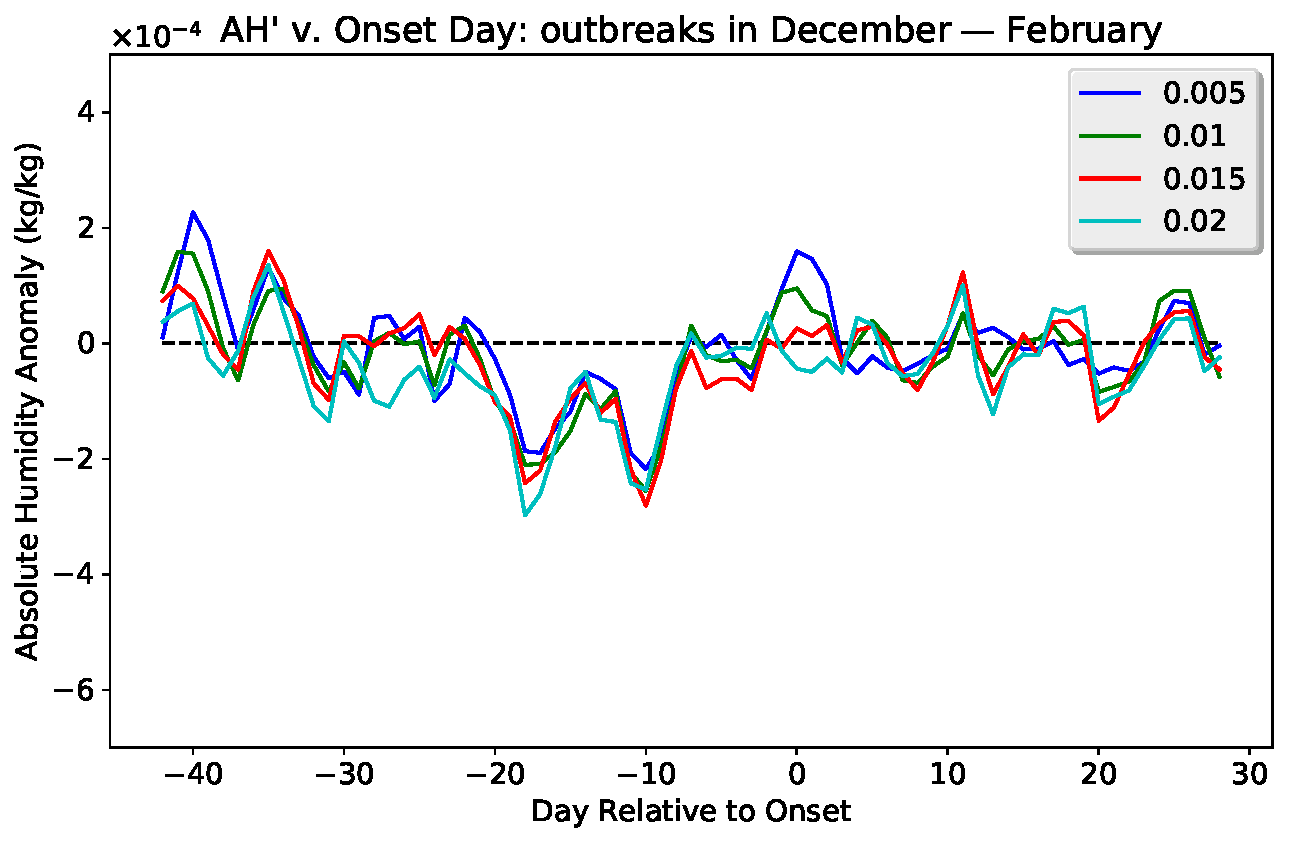
\includegraphics[width = 3in]{graphs/usa_winter12-2.pdf}\label{usa_12_2}} &
			%\subfloat[]{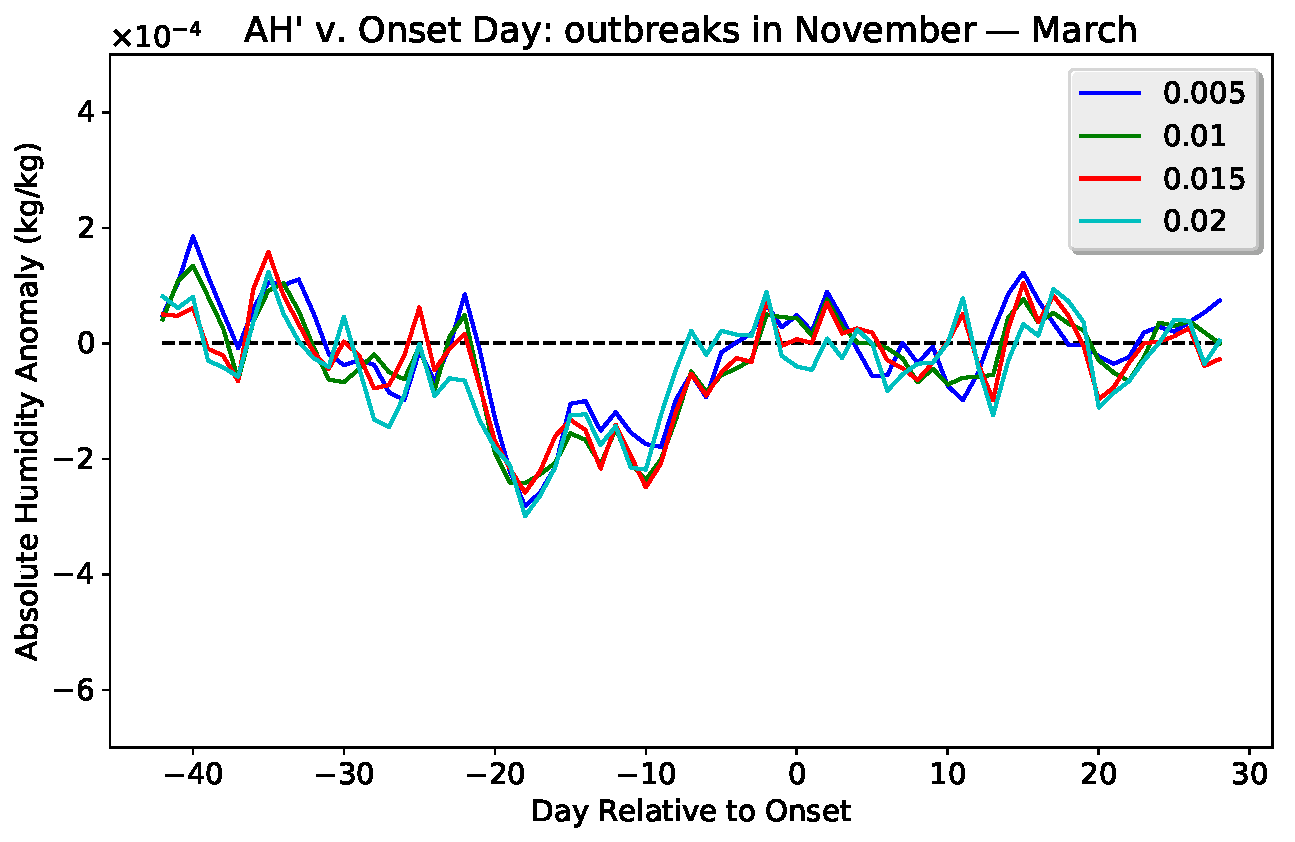
\includegraphics[width = 3in]{graphs/usa_winter11-3.pdf}\label{usa_11_3}}\\
			%\subfloat[]{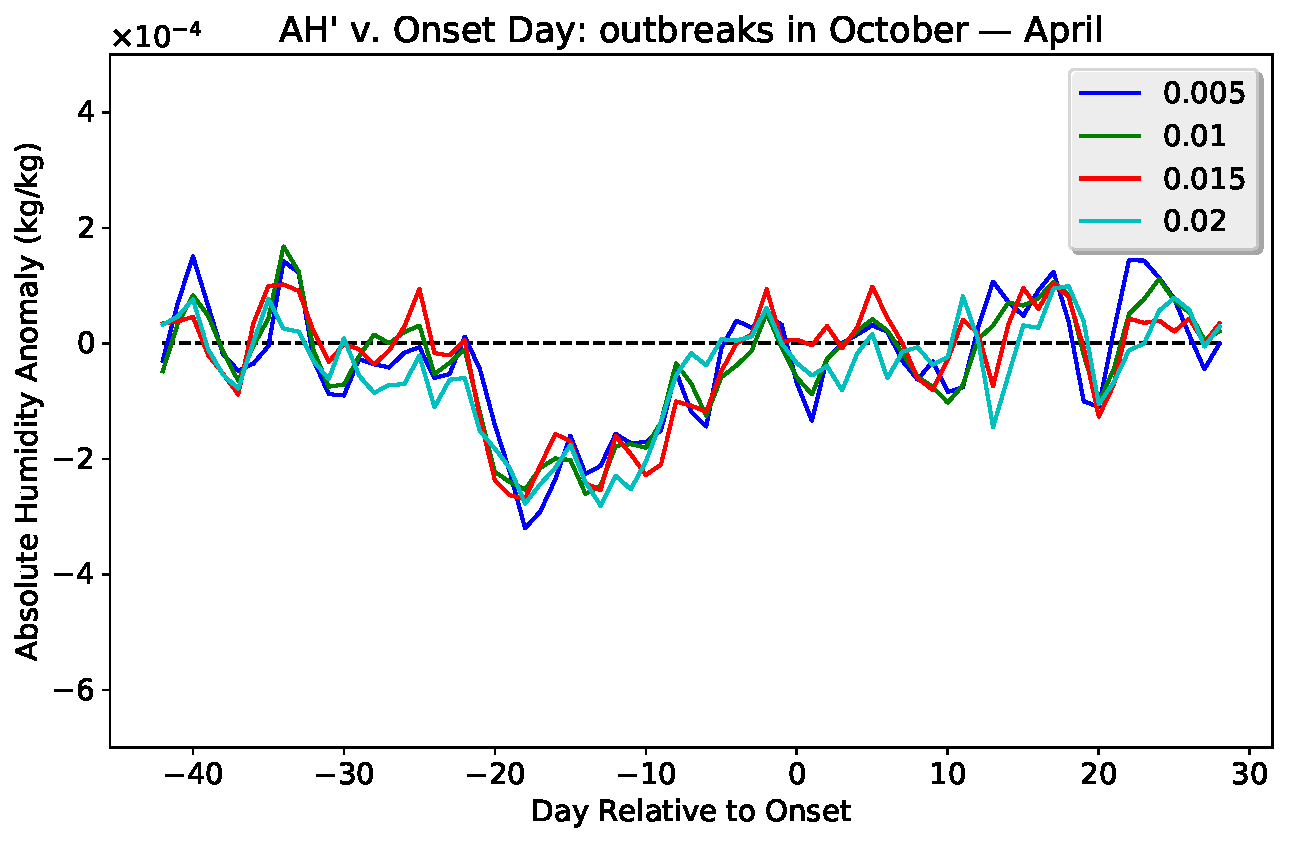
\includegraphics[width = 3in]{graphs/usa_winter10-4.pdf}\label{usa_10_4}} &
			\subfloat[]{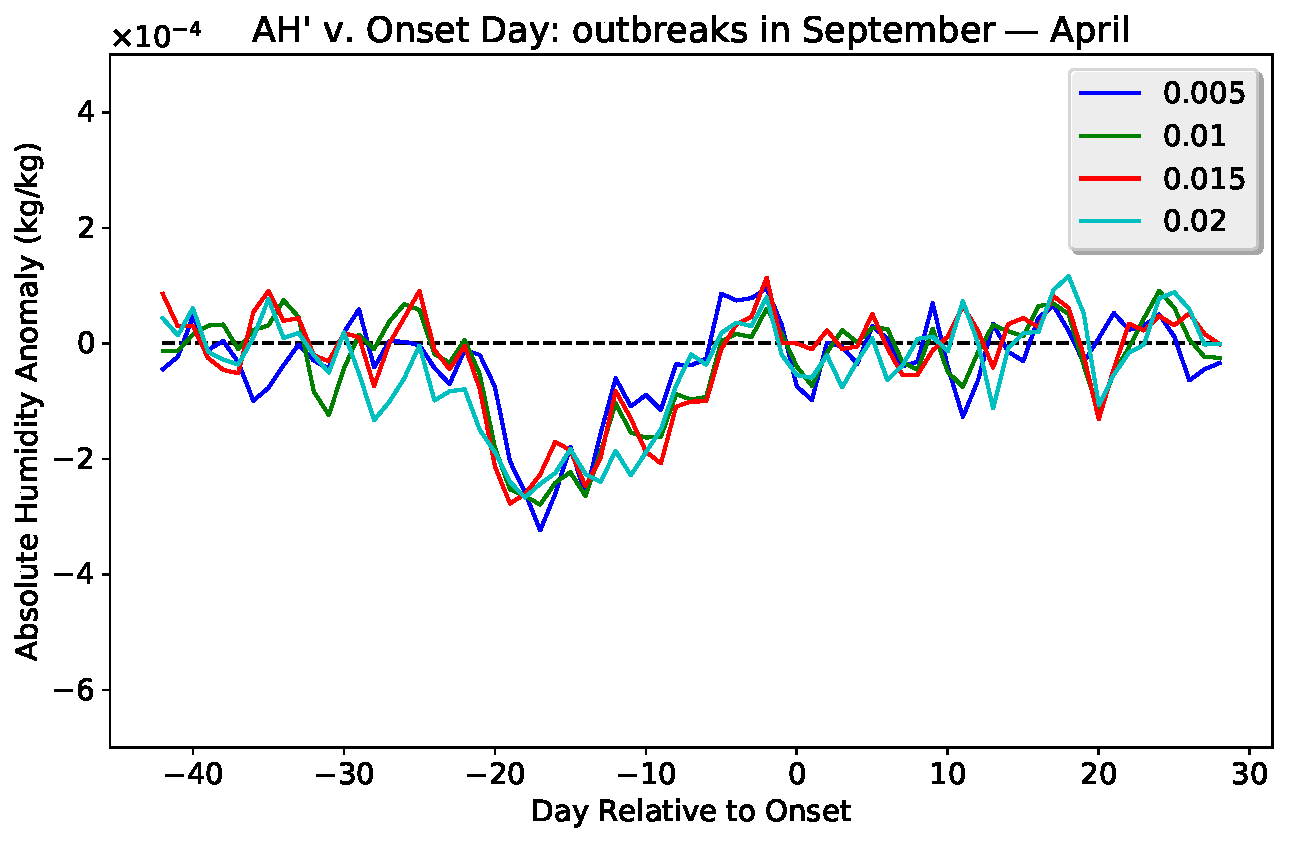
\includegraphics[width = 3in]{graphs/usa_winter9-4.pdf}\label{usa_9_4}}\\
		\end{tabular}
		\caption{$AH'$ associated with the observed onset of epidemic influenza for different onset determination criteria (two distinct wintertime seasons and four epidemic thresholds).}
		\label{figure:usa}
	\end{center}	
\end{figure}

In figure~\ref{figure:usa} one can see the dynamics of $AH'$ during six weeks before the onset and four weeks after it, averaged by all the $AH'$ datasets in the seasons when the influenza onset was detected. The solid lines show the results corresponding to different onset detection criteria --- the corresponding $P\& I$ mortality levels taken as thresholds are given in the legends. The dashed line shows $AH'$ = 0. The number of detected outbreaks obviously depends heavily on the choice of an onset threshold. Depending on the threshold level used, 1185~--~1402 epidemics were detected among 1470 theoretically possible (30 winters each for the 48 contiguous states plus the District of Columbia). The two graphs in the figure \ref{figure:usa} correspond to different definition of a winter period (i.e. the time period during a season when the $P\&I$ mortality exceeding the threshold is considered to indicate an onset). Variation of winter period definition changes the total amount of detected outbreaks as well as shifts the onset dates. 

The most pronounced $AH'$ anomaly is observed in figure~\ref{usa_9_4} when a wintertime period is set to September --- April. However, in this case the corresponding overall number of detected epidemics is as large as 1357~--~1467, depending on the thresholds. It seems implausible that influenza epidemics happened almost every winter, thus the correctness of the result may be put under doubt.
 
We can conclude that the graphs produced by the implemented algorithm are close to the ones demonstrated in \cite{shaman2010absolute}. Particularly, for all four winter intervals considered (two graphs were omitted for the sake of saving space), a visually seen $AH'$ anomaly is observed at some moment between the day -7 and day -20 (prior to onset).

\begin{figure}[htpb]
	\begin{center}
		\begin{tabular}{cc}
			\subfloat[]{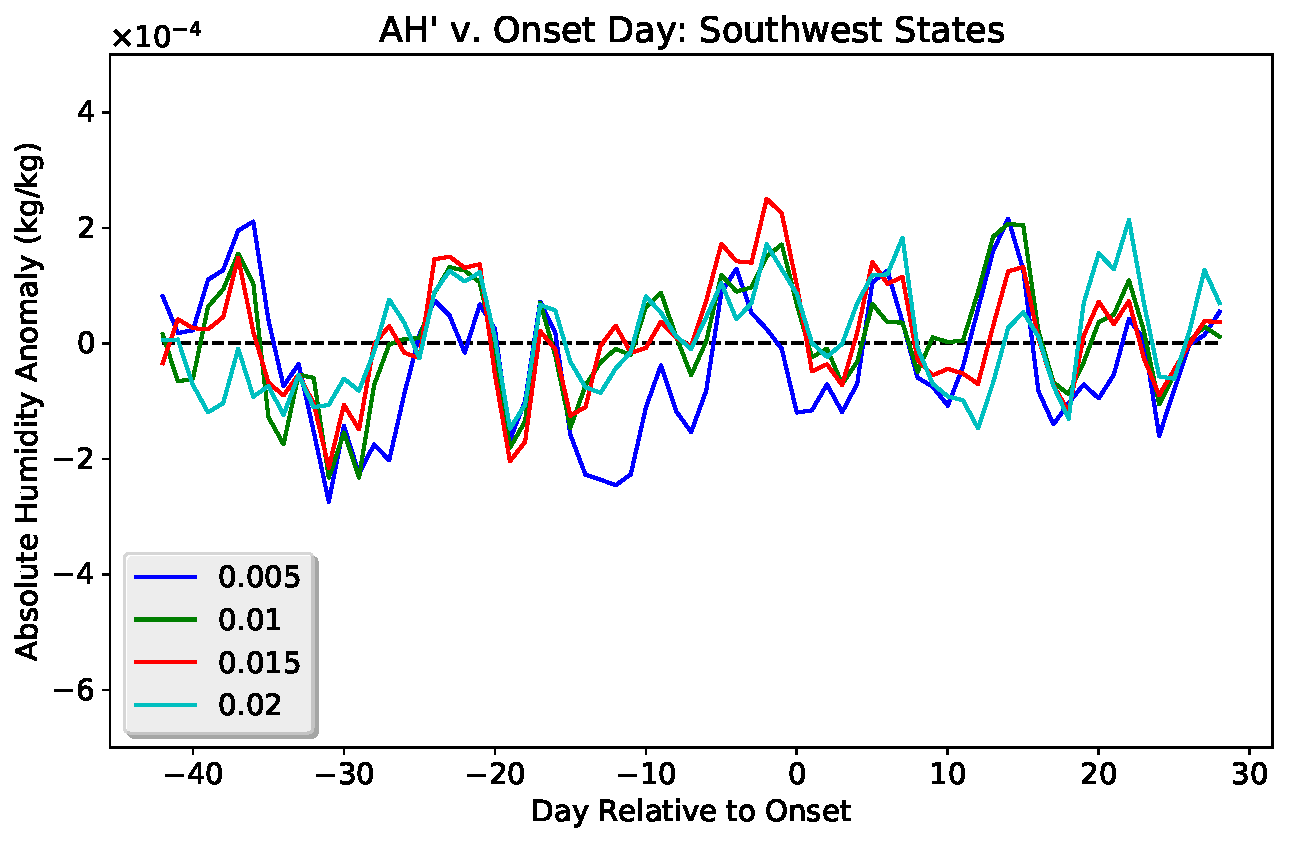
\includegraphics[width = 3in]{graphs/usa_winter10-4_sw.pdf}\label{usa_sw}} &
			\subfloat[]{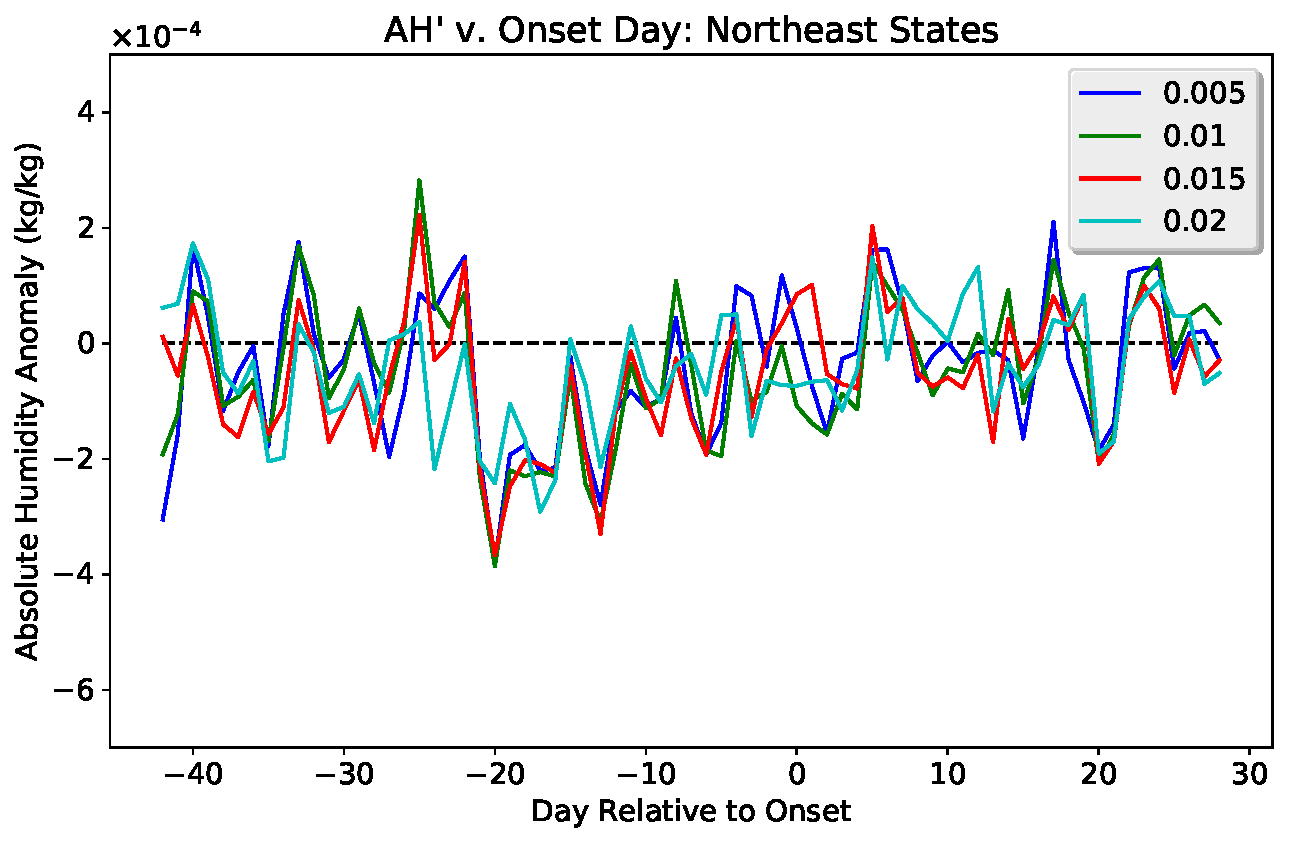
\includegraphics[width = 3in]{graphs/usa_winter10-4_ne.pdf}\label{usa_ne}}\\
			
			\subfloat[]{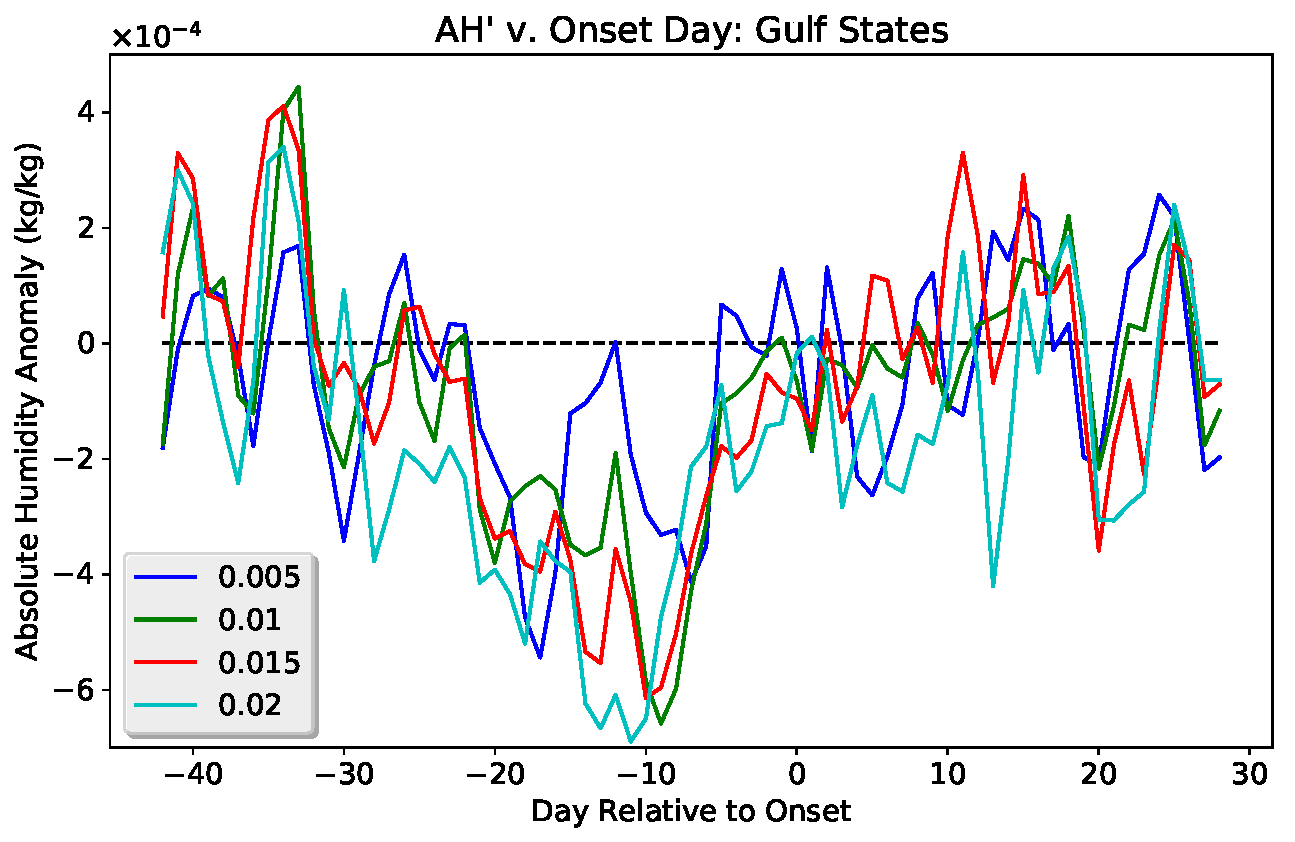
\includegraphics[width = 3in]{graphs/usa_winter10-4_gulf.pdf}\label{usa_gulf}} &
			\subfloat[]{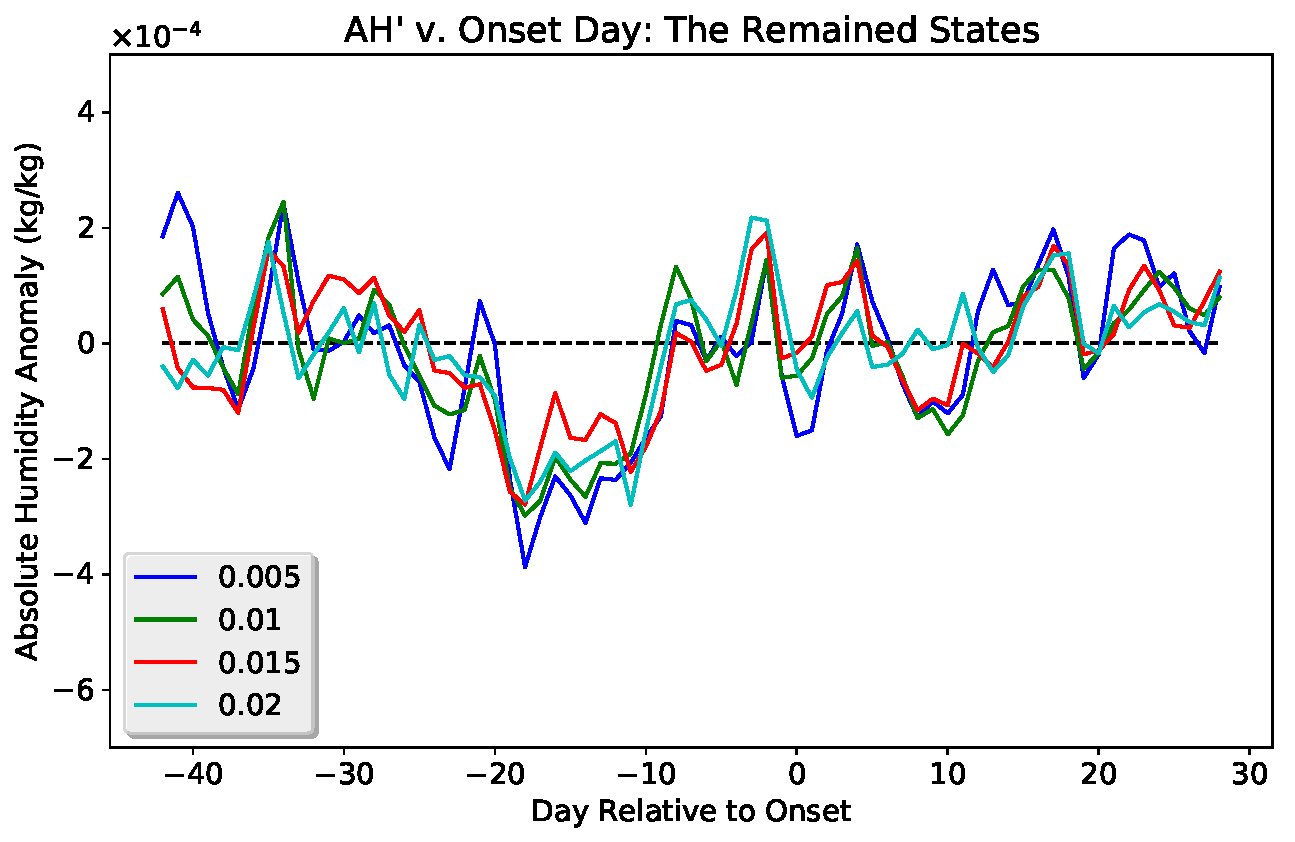
\includegraphics[width = 3in]{graphs/usa_winter10-4_the_rest.pdf}\label{usa_rest}}\\
		\end{tabular}
		\caption{Averaged $AH'$ dynamics for separate US regions}
		\label{figure:usa_regions}
	\end{center}	
\end{figure}


\begin{table}[htpb]\small
	\begin{center}
		\begin{tabular}{lrrrr}
		\hline
		State group	& Southwest & Northeast & Gulf region & The rest  \\
			\hline      
			Total onset number, $n$ & 132 & 361 & 272 & 571 \\
			\hline			
			p-value			& {\color{red} $0.525$} & { $<0.01$} & { $<0.01$} & { $0.022$}  \\			
			\hline			
		\end{tabular}
		\caption{Welch's t-test results for US state groups, epidemic threshold level $0.02 $. The results which \textbf{do not} correspond to statistically significant $AH'$ drops are marked with red.}
		\label{table:us_state_groups}
	\end{center}
\end{table}

%\label{sect:grouping} 
\paragraph{Reproducing the results for state groups.}
As the averaging of absolute humidity data goes over the whole territory of the USA, it is not very clear which part of the country gives a greater contribution to the humidity anomaly prior to onset. In \cite{shaman2010absolute} the authors addressed this issue by conducting the data analysis separately for four regions of the country: the Southwest (Arizona, Colorado, Nevada, New Mexico, and Utah), the Northeast (Connecticut, the District of Columbia, Delaware, Maine, Maryland, Massachusetts, New Hampshire, New Jersey, New York, Pennsylvania, Rhode Island, Vermont, and West Virginia); the Gulf region (Alabama, Arkansas, Florida, Georgia, Kentucky, Louisiana, Mississippi, North Carolina, South Carolina, Tennessee, and Virginia), and the rest of the states (21 in overall). Texas and California were excluded from the regional analysis due to their large geographic size and a consequent large variations in AH. The corresponding figures for the mentioned regions obtained by our algorithm are shown in fig.~\ref{usa_sw}--\ref{usa_rest}. As it can be seen from the pictures, the distinct $AH'$ anomaly before the onset is not detectable for the group of southwestern US states.

The results of statistical tests (see table \ref{table:us_state_groups}) also confirm the original conclusions.

\begin{figure}[htpb]
	\begin{center}
		\begin{tabular}{cc}
			\subfloat[]{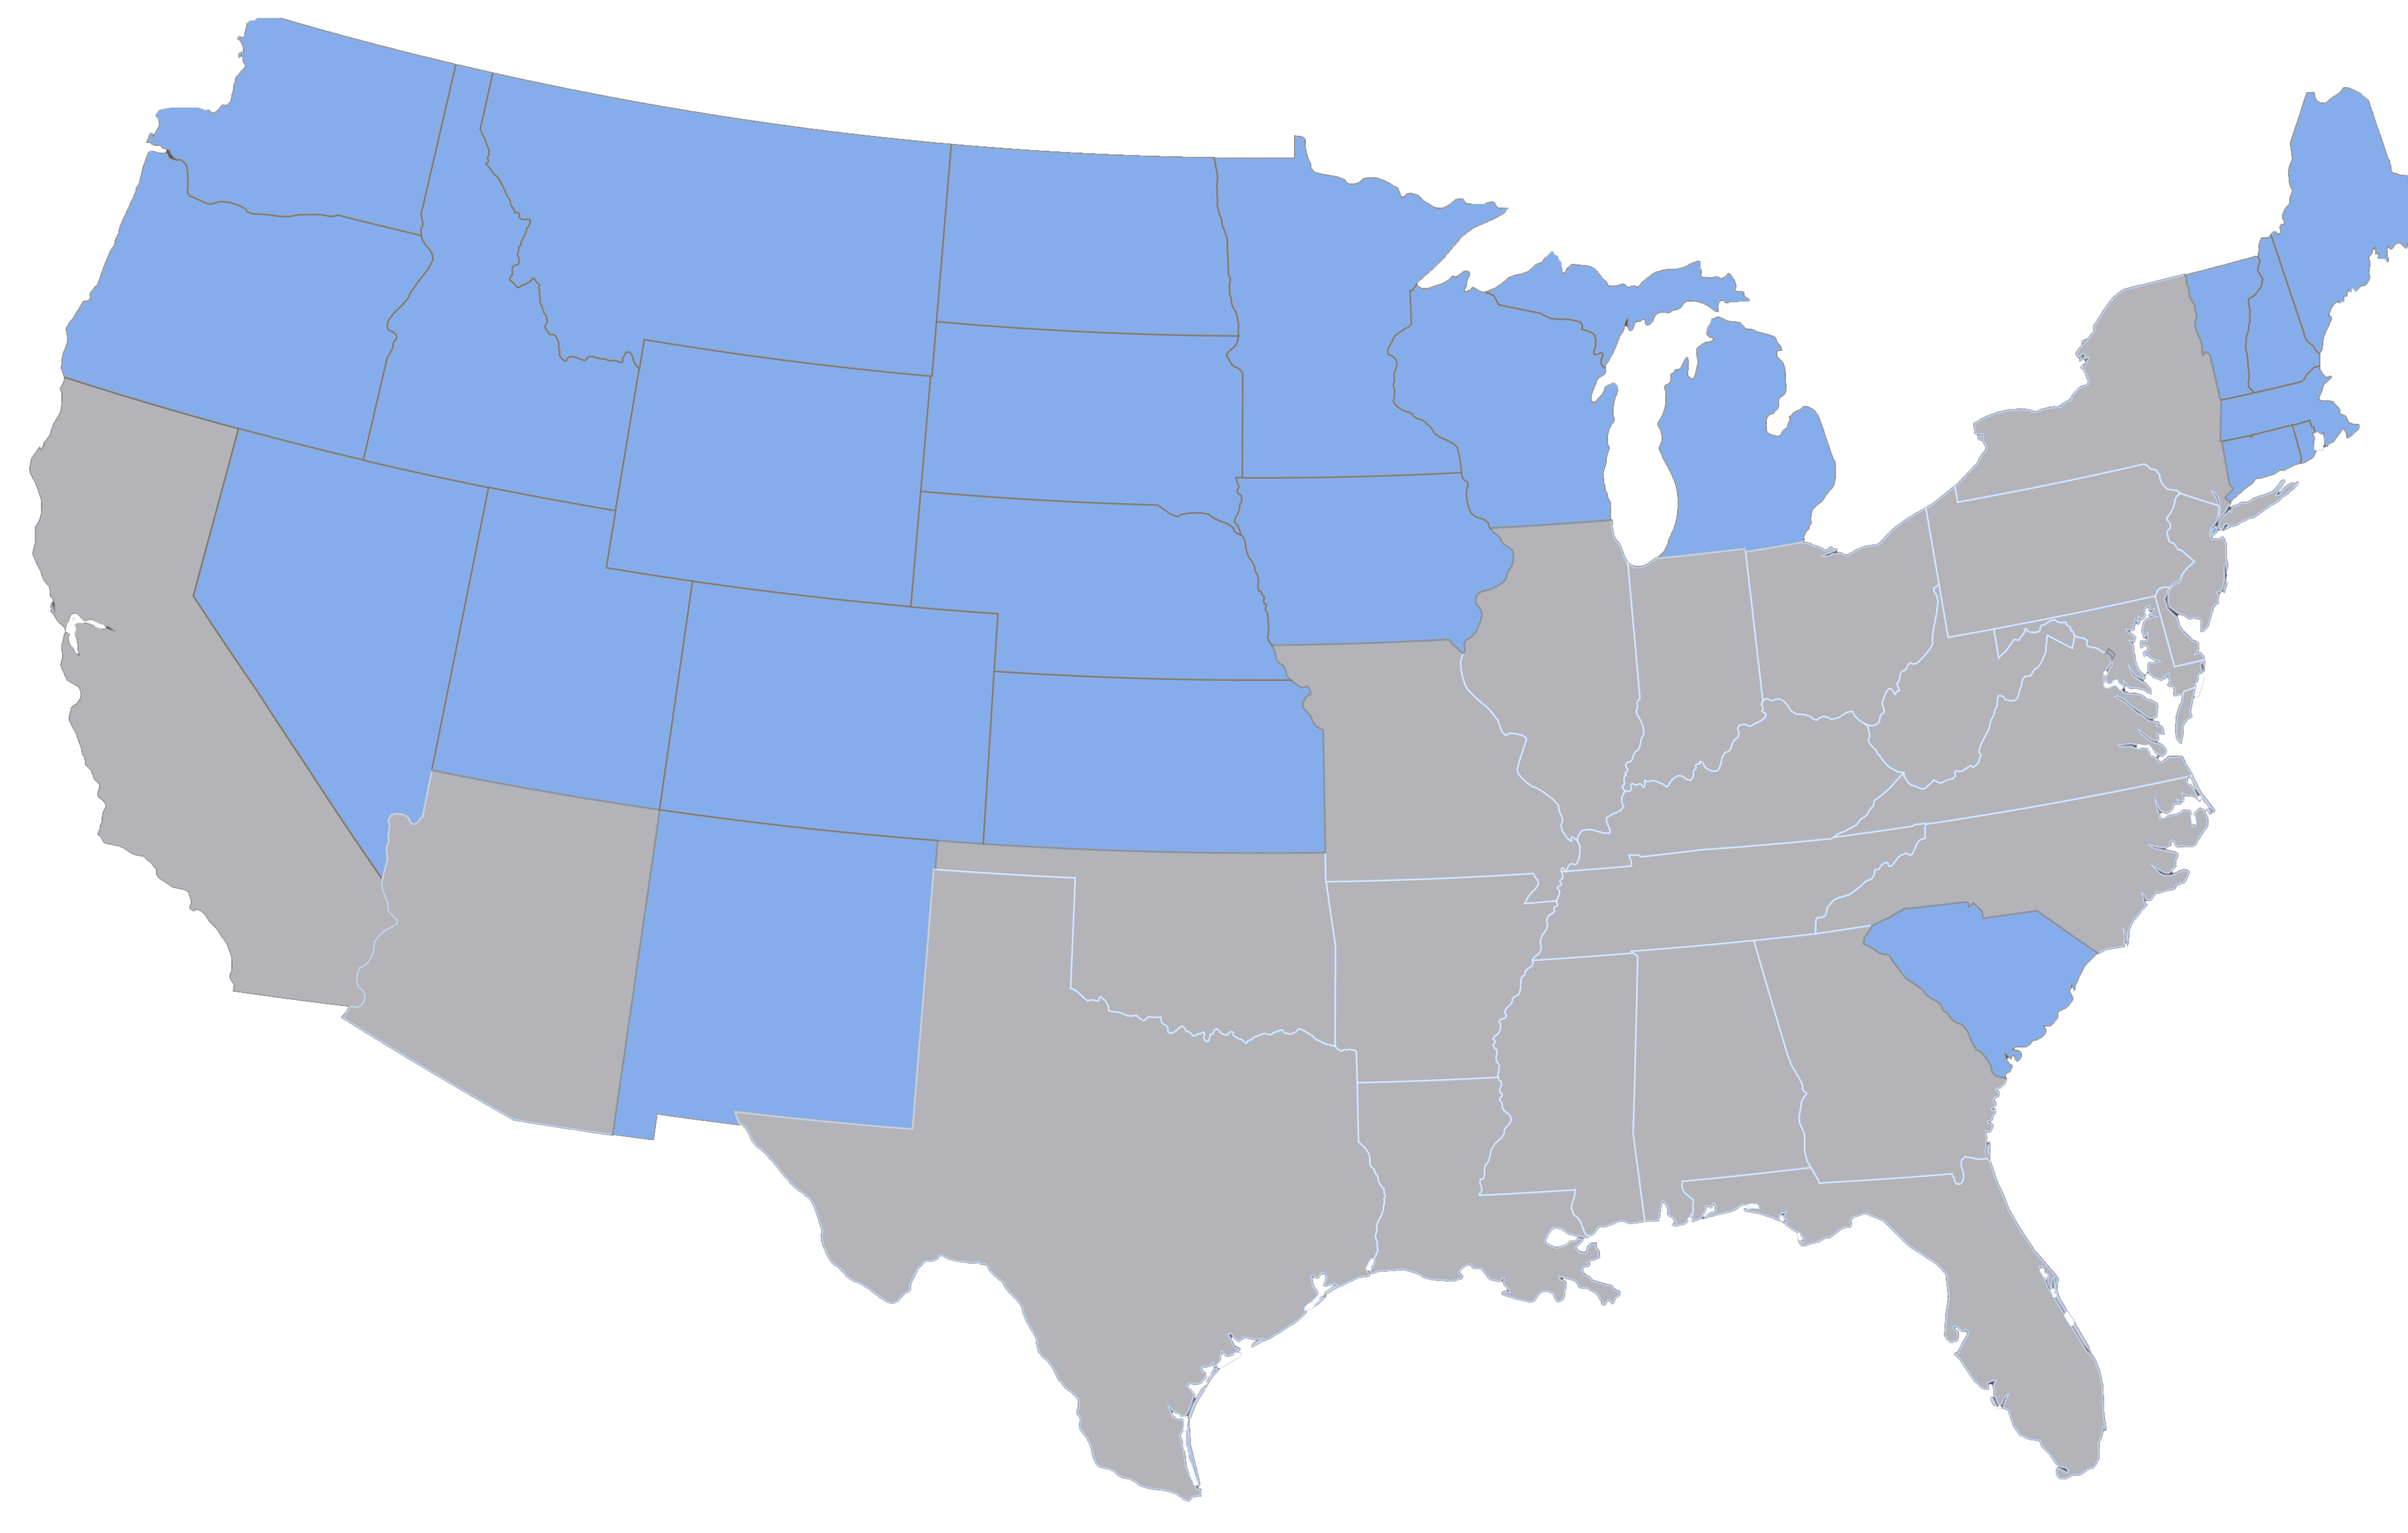
\includegraphics[width = 3in]{graphs/usa_top.png}\label{usa_top_ah_states}} &
			\subfloat[]{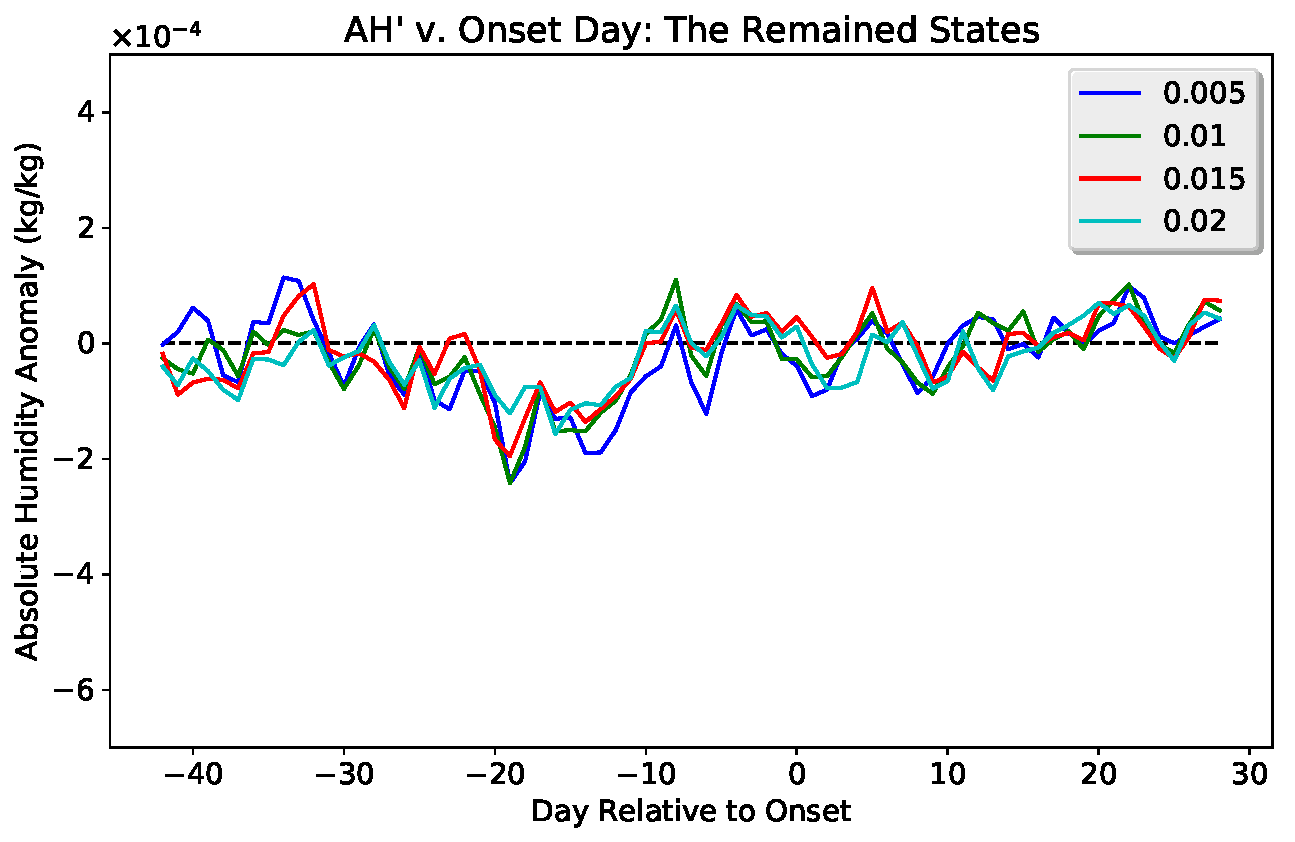
\includegraphics[width = 3in]{graphs/usa_top.pdf}\label{usa_top}}\\
		\end{tabular}
		\caption{(a): A map depicting the grouping of US states for $k=25$, the group A is drawn in gray and the group B is blue.	(b): Dynamics of $AH'$ averaged for the 6 wk prior and 4 wk following the onset, states of group B.
		}
		\label{figure:usa_top}
	\end{center}
\end{figure}

\begin{table}[htbp]\small
	\begin{center}
		\begin{tabular}{lrrrrrrrrr}
			\hline
			$k$		& 0 & 1 & 2 & 3 & 4 & 5 & 6 & 7 & 8\\
			\hline
			p-value	& $<0.01$ & $<0.01$ & $<0.01$ & $<0.01$ & $<0.01$ & 0.020 & 0.026 & 0.028 & 0.045 \\
			\hline\hline
			$k$		& {9} & {10} & {11} & {12} & {13} & {14} & {15} & {16} & {17}\\
			\hline
			p-value	& {\color{red} 0.071} & {\color{red} 0.142} & {\color{red} 0.247} & {\color{red} 0.26216} & {\color{red} 0.26352} & {\color{red} 0.26322} & {\color{red} 0.34268} & {\color{red} 0.41754} & {\color{red} 0.52582}\\
			\hline
		\end{tabular}
		\caption{Welch's t-test results for different sizes $k$ of the group A. The results which \textbf{do not} correspond to statistically significant $AH'$ drops are marked with red. }
		\label{table:top}
	\end{center}
\end{table}

\paragraph{Regarding separate states.}

It is obvious that the averaged $AH'$ dynamics of a given region is composed of AH dynamics in separate states, and their contribution to the drops of $AH'$ is not equal. For example, in Mississippi $AH'$ drops down to $-0.00212$ in period from $19$ to $10$ days prior to onset, which is $7$ times greater by absolute value than the minimum $AH'$ drop over all contiguous states. Thus, to assess the impact of absolute humidity anomaly in each of the states towards the overall $AH'$ drop we performed the following data analysis. All the states were sorted by minimal absolute value of $AH'$ in the mentioned period. Let's name ``group A'' the group of $k$ states with most prominent $AH'$ anomaly, whereas the remaining states constitute the group B. If we compare visually the graphs of averaged $AH'$ dynamics in a group B for $k=0$ (averaging by all the states) and $k = 21$ (the data of 21 states is excluded from the averaging procedure), they contain a distinct and almost similar $AH'$ drop. However, if $k$ reaches $25$, the $AH'$ anomaly becomes hardly distinguishable (see figure~\ref{figure:usa_top}).


%------------------------------------------------------------------------------

To support the visual observations we performed the statistical tests for different values of $k$. The following procedure was employed:
\begin{itemize}
	\item Let $B$ be a set of states sorted in ascending order by minimal $AH'$ value within 28-days period prior to onset. 
	\item For each state $S$ in $B$:
	\begin{itemize}		
		\item Generate arbitrary and preonset $AH'$ samples
			for the group of states $B$
		\item Perform  Welch's t-test to accept or reject the hypothesis of the equivalence of average sample means.
		\item Remove $S$ from the group $B$.
	\end{itemize}
\end{itemize}

The results demonstrated in table~\ref{table:top} show the growth of $p-$value with the growth of $k$. One can see that starting from $k = 9$ the null hypothesis of identical sample means is accepted, which means that $AH'$ drop is claimed to be insignificant.

We also performed the same statistical analysis for the data on separate US states. Surprisingly, only three distinct states, -- namely, Alabama, Georgia and Louisiana, -- demonstrated significant $AH'$ drops.


\subsection{Influenza onsets in Russia}

\paragraph{Data.}
The $AH$ dataset contains daily absolute humidity ($AH$) in the three biggest Russian cities, -- Moscow, Saint-Petersburg and Novosibirsk, -- from 1985 to 2015. The epidemiological data consists of two datasets. The first one included weekly incidence of acute respiratory infections from June, 1985 to May, 2015 (29 epidemic seasons). The second one, for the same time period, is a binary array: '1' means officially declared influenza epidemic in the corresponding week, and '0' means the absence of epidemics. This array, along with ARI incidence data, was provided by Russian Research Institute of Influenza \cite{fluinst_link}. The original ARI incidence data was converted to daily one by means of cubic interpolation and corrected for under-reporting during holidays \cite{baroyan1970computer}, \cite{Leonenko2016}.  

To form the influenza onset dates array we have used two methods:
\begin{itemize}
\item \textbf{Using external assessment.} Taking the binary array as a source of information on epidemic days in a fixed season, we considered Thursday of the first week marked with '1' to be an onset day.
\item \textbf{Using epidemic thresholds.} Similarly to the rule applied to US $P\&I$ mortality in the previous section, we consider the particular date to be a date of influenza onset in the particular location if it belonged to wintertime period and the corresponding ARI incidence had been at or above a prescribed threshold level during the two preceding weeks. The threshold levels for ARI incidence were taken in such a way that the total number of detected onsets was close to the number obtained by the external assessment (i.e. the official number of flu epidemics provided by Russian healthcare organs). 
\end{itemize}

The binary array contained $72$ epidemics in total (out of $29 \cdot 3 = 87$ theoretically possible epidemics). The corresponding epidemic threshold level appeared to be 5 new flu cases/100,000 people/day for the three cities combined (resulting in 70 detected epidemics). The $AH'$ graphs for the both onset array generation algorithms are presented in figure~\ref{figure:rf}. For both cases there is no visual evidence of $AH'$ drops, and the statistic test proves this: for the left graph $p$-value $\approx 0.78$, and for the thresholds on the right graph $p=0.286$, $0.156$ and $0.15$ correspondingly (see also table \ref{table:rf_ttest}).


\begin{figure}
	\begin{center}
		\begin{tabular}{cc}									
			\subfloat[]{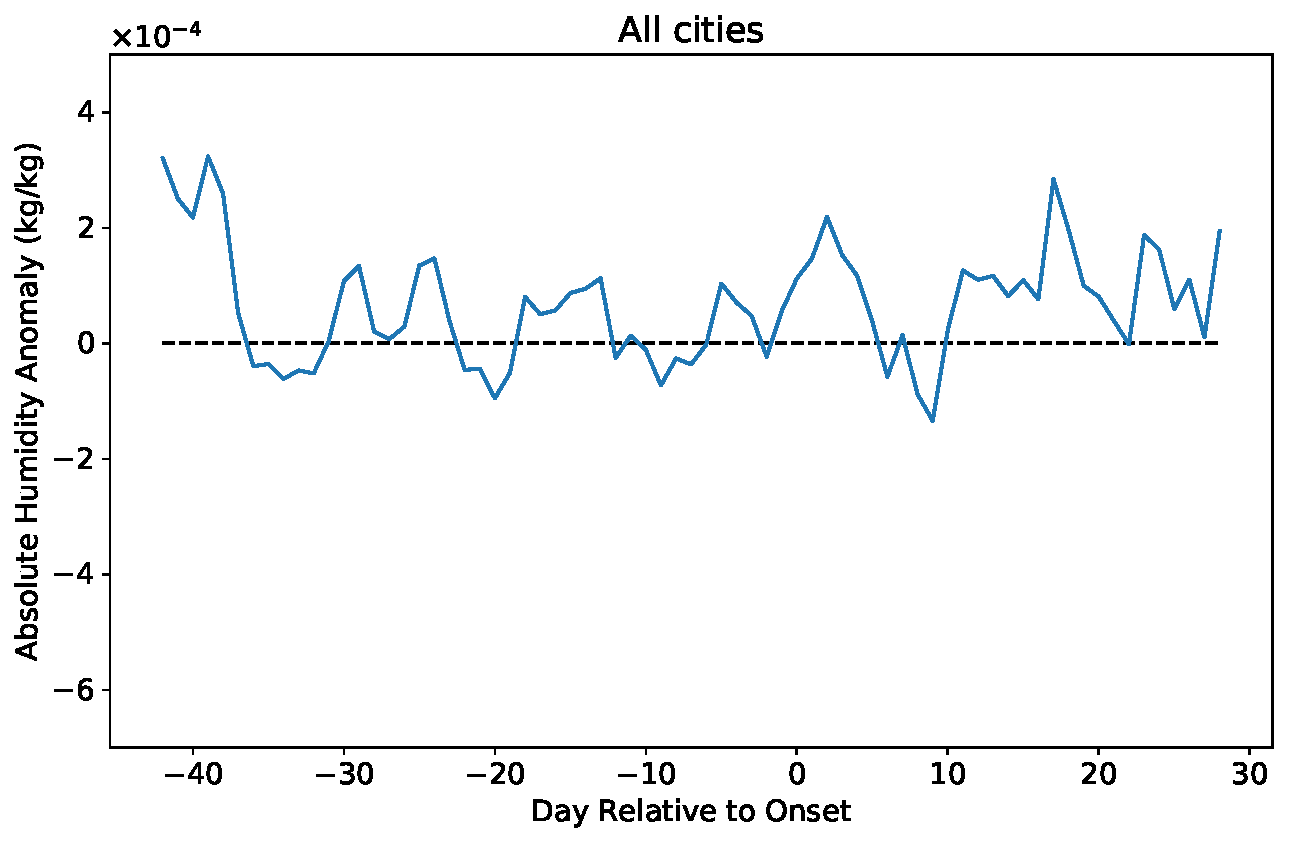
\includegraphics[width = 3in]{graphs/rf_spb,msk,nsk.pdf}\label{rf_all}} &
			\subfloat[]{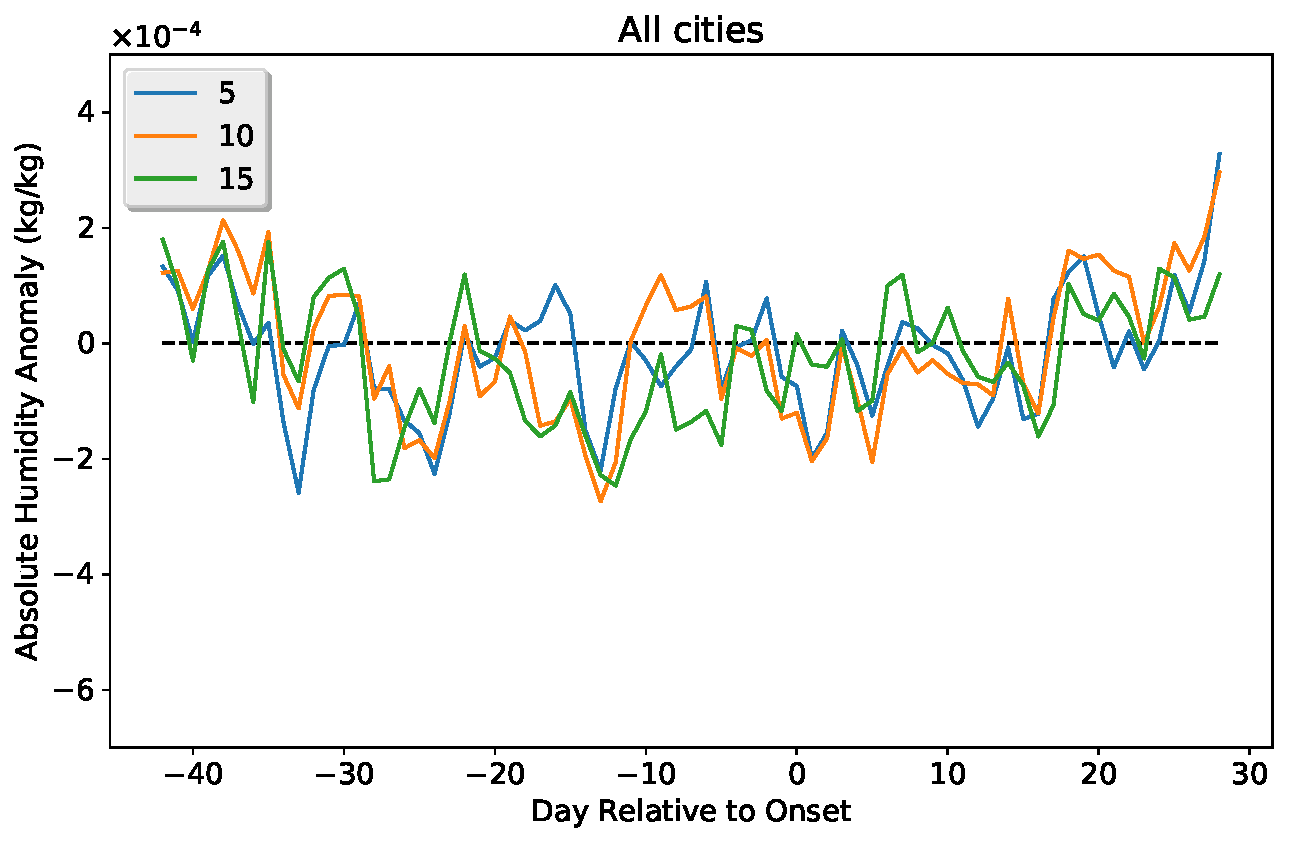
\includegraphics[width = 3in]{graphs/rf_m_spb,msk,nsk_winter11-3_threshold5-15.pdf}\label{rf_all_morbidity}}\\
		\end{tabular}
		\caption{Dynamics of $AH'$ averaged for the 6 wk prior and 4 wk following the onset for three Russian cities: (a) onsets are taken from external sources; (b) onsets are detected using incidence thresholds.}
		\label{figure:rf}
	\end{center}
\end{figure}

\begin{figure}[htbp]
	\begin{center}
		\begin{tabular}{cc}
			\subfloat[]{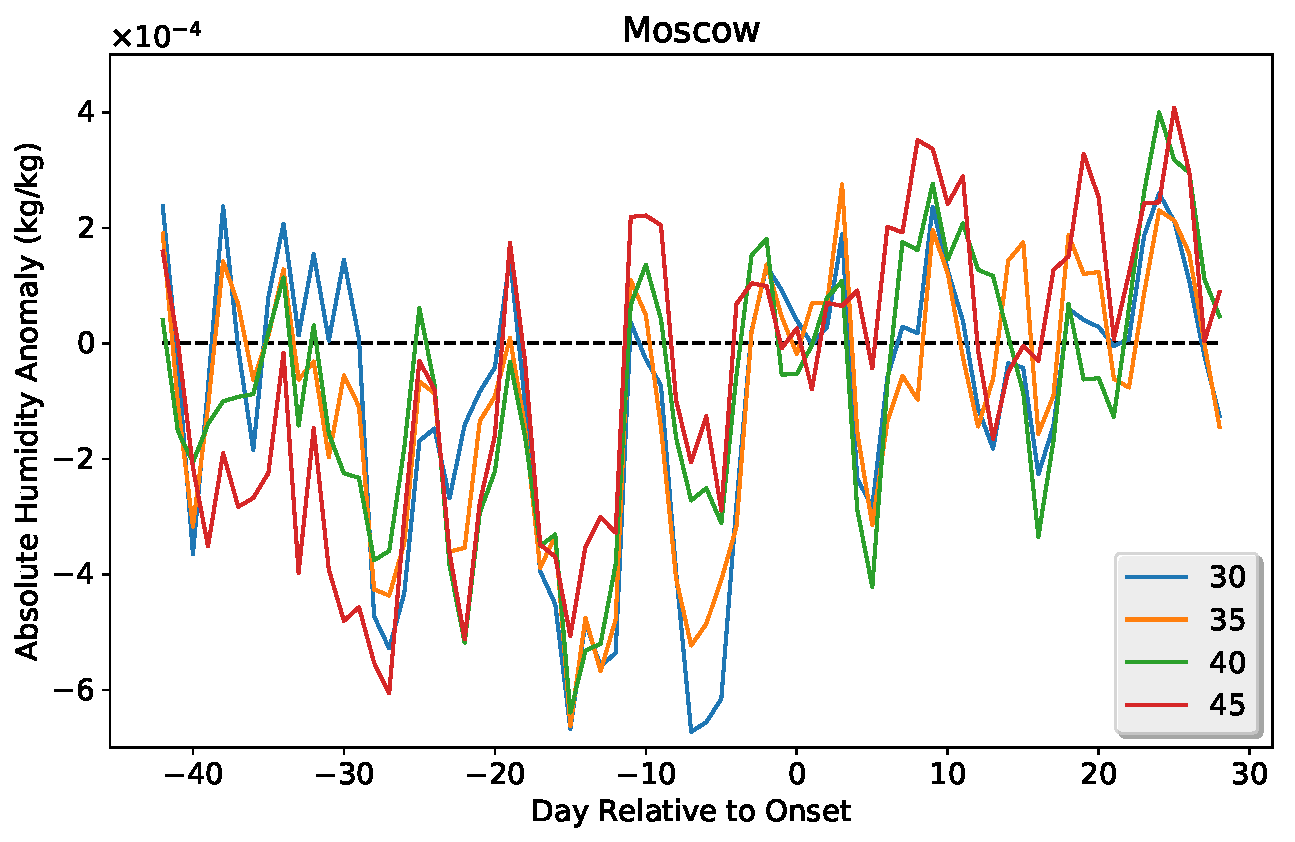
\includegraphics[width = 3in]{graphs/rf_m_Moscow_winter11-3_threshold30-45.pdf}\label{rf_msk_morbidity_ext}} &
			\subfloat[]{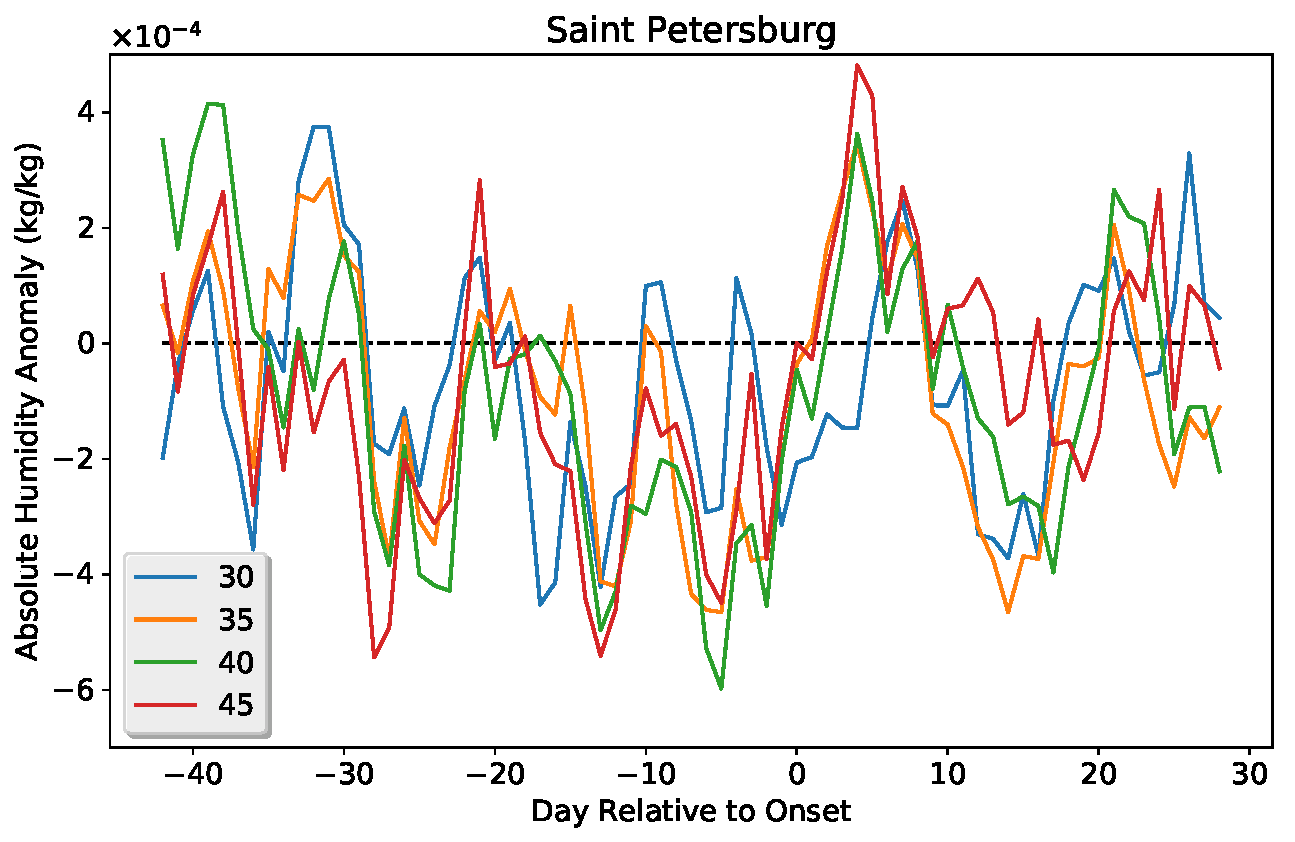
\includegraphics[width = 3in]{graphs/rf_m_SaintPetersburg_winter11-3_threshold30-45.pdf}\label{rf_spb_morbidity_ext}}\\
			
			\subfloat[]{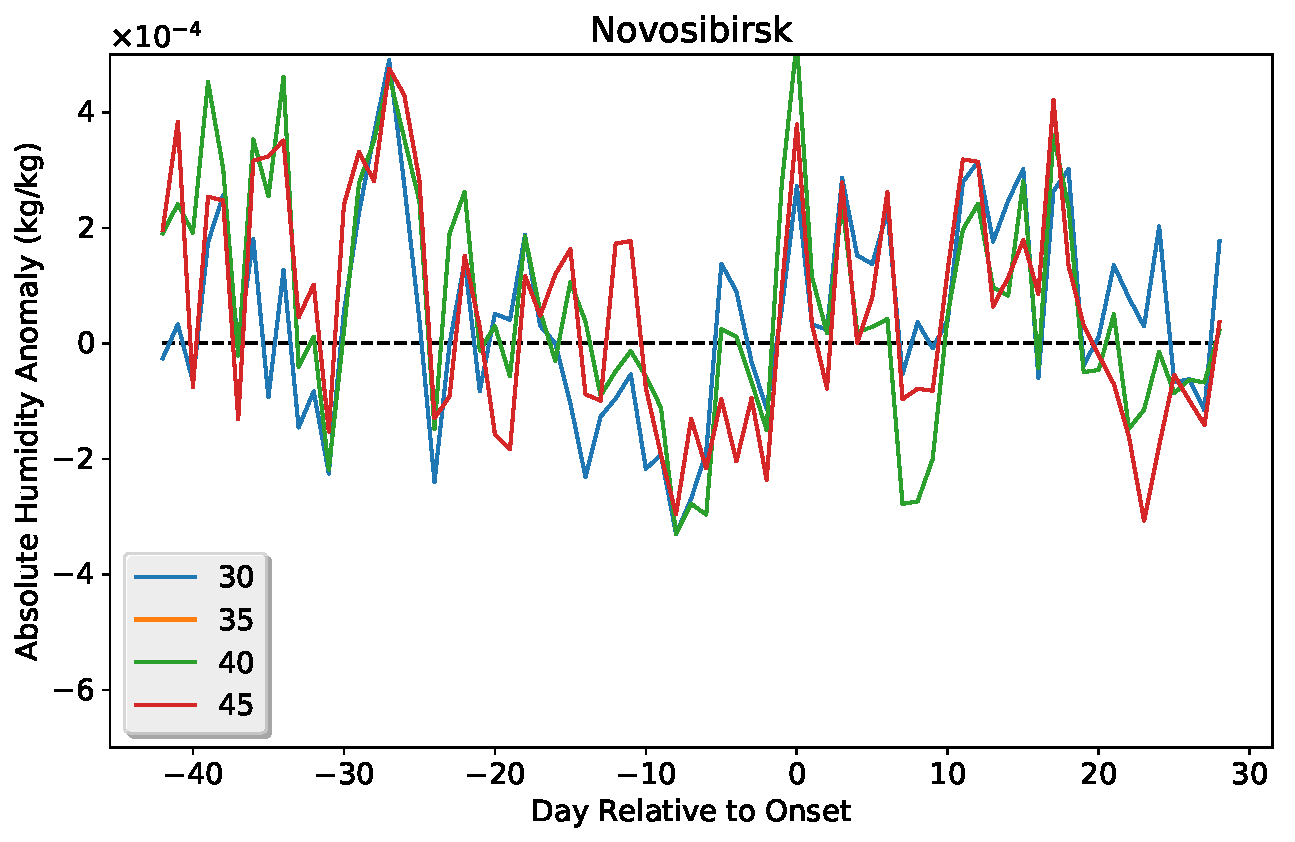
\includegraphics[width = 3in]{graphs/rf_m_Novosibirsk_winter11-3_threshold30-45.pdf}\label{rf_nsk_morbidity_ext}} &
			\subfloat[]{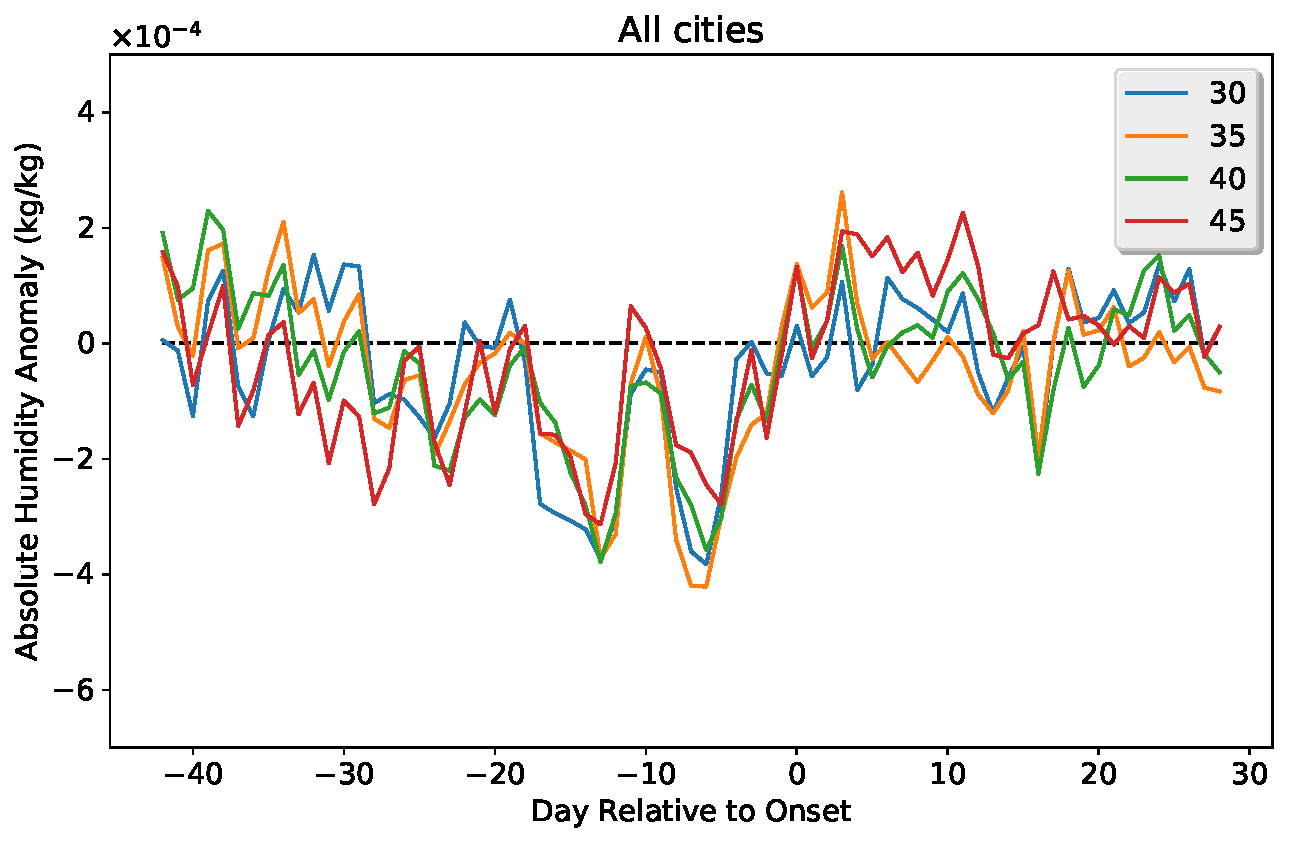
\includegraphics[width = 3in]{graphs/rf_m_spb,msk,nsk_winter11-3_threshold30-45.pdf}\label{rf_all_morbidity_ext}}\\
		\end{tabular}
		\caption{Dynamics of $AH'$ averaged for the 6 wk prior and
			4 wk following the onset, high epidemic thresholds}
		\label{figure:rf_morbidity_ext}
	\end{center}	
\end{figure}

\begin{table}[tb]\small
	\begin{center}
		\begin{tabular}{lrrrrrrrr}
			\hline
			Threshold		& 5 & 10 & 15 & 20 & 25 & 28 & 30 & 35 \\
			\hline      
			p-value			& {\color{red} 0.28639} & {\color{red} 0.15597} & {\color{red} 0.05876} & {\color{red} 0.1501} & {\color{red} 0.09052} & 0.03724 & 0.02619 & 0.02523 \\
			\hline
			Total onset number, $n$ & 70 & 69 & 62 & 59 & 53 & 51 & 50 & 47 \\
			\hline
			\hline
			Threshold		& 40 & 43 & 44 & 45 & 50 \\
			\hline      
			p-value			& 0.03144 & 0.0405 & {\color{red} 0.07254} & {\color{red} 0.06196} & {\color{red} 0.14596} \\
			\hline
			Total onset number, $n$ & 45 & 44 & 43 & 43 & 39 \\
		\end{tabular}
		\caption{Welch's t-test results for Russian cities, the onsets determined by incidence threshold}
		\label{table:rf_ttest}
	\end{center}
\end{table}

An interesting fact was revealed when we performed tests with higher threshold levels. Starting from the threshold level $28 $ we observe a distinct $AH'$ drop before the onsets in the graphs (see figure~\ref{figure:rf_morbidity_ext}) and the corresponding {p-values} are below 0.05. A significant $AH'$ drop is demonstrated for the thresholds from $28 $ to $43 $. With further increasing of the threshold level the drops again cease to exist. 


\begin{figure}[htbp]
	\begin{center}
		\begin{tabular}{cc}
			\subfloat[]{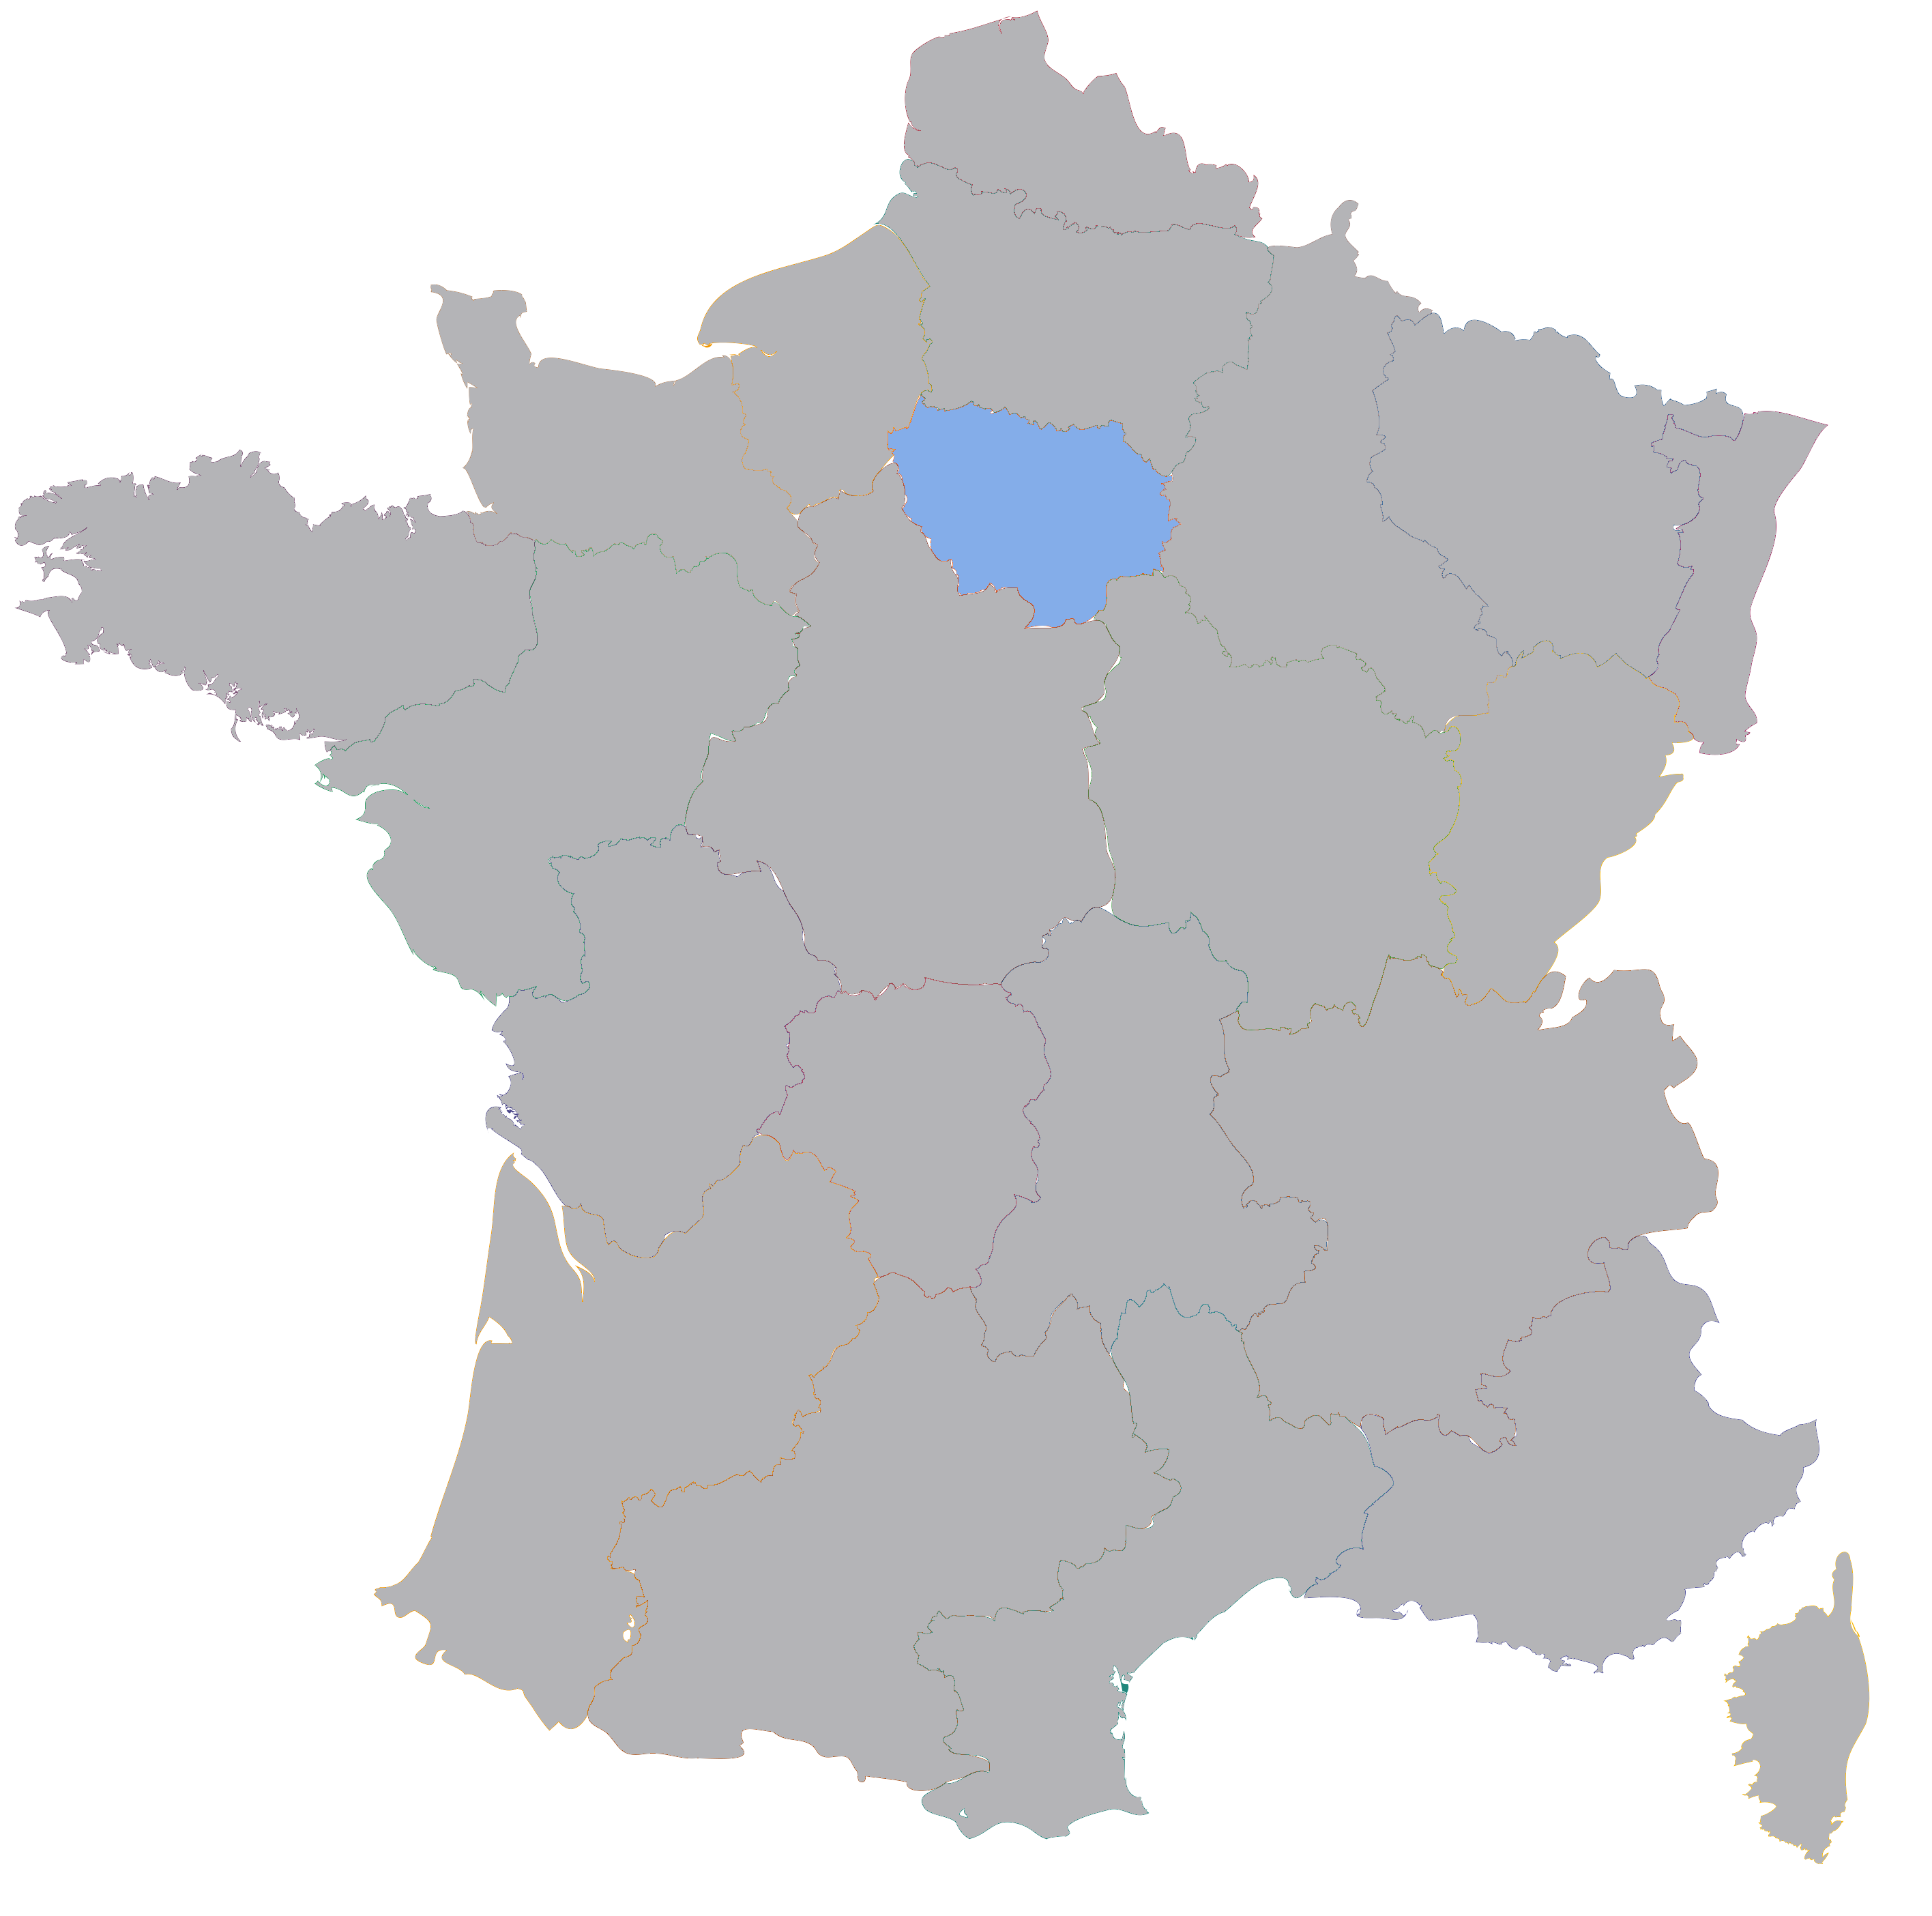
\includegraphics[width = 2in]{graphs/ile_de_france.png}} &
			\subfloat[]{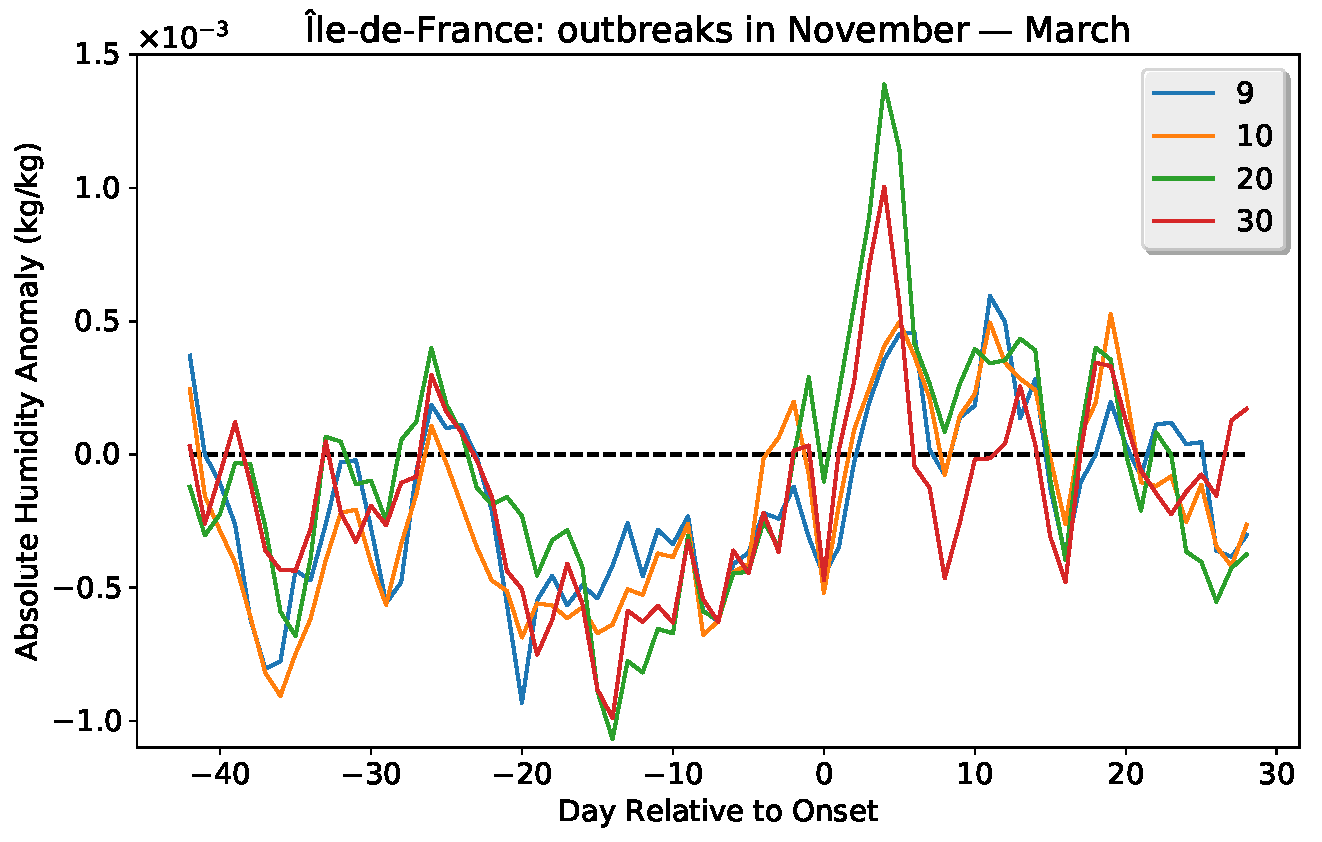
\includegraphics[width = 3in]{graphs/paris_winter11-3_threshold30.pdf}}
		\end{tabular}
		\caption{(a): Ile-de-France region on the map of France;
			(b): dynamics of $AH'$ averaged for the 6 wk prior and
			4 wk following the onset, Ile-de-France}
		\label{figure:paris}
	\end{center}
\end{figure}

\begin{table}[htbp]\small
	\begin{center}
		\begin{tabular}{lrrrrrrrr}
			\hline
			Threshold			& 1 & 2 & 3 & 4 & 5 & 6 & 7 & 8 \\
			\hline
			p-value				& {\color{red}0.15874} & {\color{red}0.11891} & {\color{red}0.08969} & 0.0382 & 0.049 & {\color{red}0.05086} & {\color{red}0.05241} & {\color{red}0.09705} \\
			\hline
			Total onset number, $n$	& 25 & 25 & 24 & 22 & 21 & 21 & 21 & 21 \\
			\hline\hline
			Threshold			& 9 & 10 & 12 & 15 & 17 &20 & 25 & 30 \\
			\hline
			p-value				& 0.04526 & 0.04712 & 0.02676 & 0.0209 & 0.02123 & 0.04627 & 0.04445 & 0.03916 \\
			\hline
			Total onset number, $n$	& 20 & 18 & 17 & 17 & 17 & 15 & 15 & 12 \\
			\hline
		\end{tabular}
		\caption{Welch's t-test results for Ile-de-France, depending on morbidity threshold}
		\label{table:paris}
	\end{center}
\end{table}

\subsection{Influenza onsets in Ile-de-France}
For the comparison purposes, we decided to test our algorithm on the absolute humidity and incidence data for Ile-de-France (includes Paris and its suburbs), 1985 -- 2015. The French epidemiological data was taken from Sentinelles surveillance network \cite{sentinelles}. Apart from the Russian data, it includes only the cases of influenza-like illness (severe ARI forms similar by symptoms to the flu) rather than all the cases of ARI. Epidemic thresholds for the onset detection algorithms were set somewhat arbitrary to correspond to ``reasonable'' number of detected epidemics. The wintertime period was assumed to start in November and end in March. The resulting detected onset number $n$ varied from 12 to 20 (of 29 possible in 1985 -- 2015 period). The graph for the resulting averaged $AH'$ is demonstrated in figure~\ref{figure:paris}

The first thing one can observe from the graph is that the $AH'$ drop is perfectly visible and, moreover, its absolute value is even greater than of the drops for the US states (see, for instance, figure \ref{usa_gulf}). Thus it is not surprising that the statistical tests demonstrate significance of the drops for incidence threshold levels above 9 new incidence cases/100000 people/day (see table~\ref{table:paris}).

\section{Discussion}

In this work we have implemented the computational algorithm which makes it possible to analyze the dynamics of absolute humidity before and after the influenza onsets. Our aim was to find out if the abnormal $AH'$ drops described by Shaman et al. could serve as harbingers of incoming influenza epidemics in the regions apart from the USA, namely, France and Russia. Also, the question was to what extent the results obtained for the US state groups are dependent on the group choice. Our conclusions can be summarized in a following way:

\begin{itemize}
\item Speaking of the USA, the most distinct $AH'$ drops before the onset happen in the southeastern states, as well as in the states in the south-west of the country which are close to the ocean (Arizona and California). At the same time, the statistical significance of the mentioned drops is reached, according to Welch's t-test, only in three states -- the latter result is rather controversial and requires further investigation.

\item The Ile-de-France region showed even more distinct drops in $AH'$ than the US states.

\item The influenza onsets in Russian cities under considerations are generally not preceded by any abnormal dynamics of $AH$. A number of experiments with Russian data in which we were able to reach statistical significance of $AH'$ drops (corresponding to the onset thresholds from $28$ to $43$) were performed using presumably unrealistic input parameter values (the resulting number of detected epidemics did not exceed $51$, which is significantly less than the number of $72$ determined by the epidemiologists).
\end{itemize}

The authors have to admit that the accuracy of the results may be somewhat undermined by the heterogeneity of the data employed (different methods of onset detection, different sizes of regions under study), uncertainty of the input (namely, the selection of epidemic threshold levels) and the possible limitations of the statistical procedure employed to detect the significant $AH'$ drops. Nevertheless, the current results allow us, somewhat speculatively, to draw a parallel between Russia, France and the US states. The preliminary hypothesis could be made that for the case of locations situated within the latitude span of the US territories (i.e., we exclude the tropics and southern hemisphere), the higher average temperatures (and thus, bigger variation in absolute humidity) and smaller distance to the seashore may lead to more pronounced drops in $AH'$ before the influenza onset. On the contrary, if the region under consideration is located to the north and far from the shore, one won't be successful in predicting influenza onsets by $AH'$ drops. The latter is the case both for the major part of the American North and the three biggest Russian cities.

As a future perspective, we think of applying the algorithm to the extended Russian ARI dataset, particularly, including the Russian cities which are situated closer to the southern seas and have milder climate (e.g., Sochi, Krasnodar, Stavropol). Perhaps, the analysis of such dataset will bring us to new interesting insights and help specify the conditions under which the $AH$ dynamics may be incorporated into flu prediction models.

%In order to ascertain the reasons of unsuccessful method application
%to Russian cities, the distribution of the
%epidemics onset, determined by a two-week deviation of morbidity (mortality)
%from a thirty-year average, was compared.
%
%It can be concluded that like entire U.S., and three regions considered
%separately, they have a plateau in the beginning of site-winter. It means
%that most onsets occur in first 5 weeks uniformly.
%As for Russia, threshold variation generates random patterns with
%similar peak in the very beginning. Greedy empiric method pushes to
%expand the scope of winter, which is logical, because in Russia's 
%winter is much longer than three month, and epidemiologic period
%could be stretched out until September to May.

% На данных РФ и Франции аномалия в общем случае не воспроизводится, кроме ряда исключений (показать выбор порога для этого).


\section{Acknowledgments}

The authors want to express their gratitude to Dr. Jeffrey Shaman both for providing the data on US P\&I Mortality and for giving his comments on the details of data analysis performed in \cite{shaman2010absolute}.


%------------------------------------------------------------------------------
%------------------------------------------------------------------------------
% Refs:
%
\label{sect:bib}
\bibliographystyle{plain}
%\bibliographystyle{alpha}
%\bibliographystyle{unsrt}
%\bibliographystyle{abbrv}
\bibliography{ivanov_leonenko}
%------------------------------------------------------------------------------

%------------------------------------------------------------------------------


%\begin{table}[tb]\small
	%\begin{center}
		%\begin{tabular}{lrr}
			%\hline
			%Site name	& \textbf{experimental} sample size & \textbf{P-value} \\
			%\hline\hline
			%Alabama & 27 & \textbf{0.02163} \\
			%\hline
			%Arizona & 26 & 0.91901 \\
			%\hline
			%Arkansas & 27 & 0.21912 \\
			%\hline
			%California & 26 & 0.46057 \\
			%\hline
			%Colorado & 27 & 0.65945 \\
			%\hline
			%Connecticut & 28 & 0.14077 \\
			%\hline
			%Delaware & 29 & 0.07496 \\
			%\hline
			%District of Columbia & 28 & 0.60343 \\
			%\hline
			%Florida & 27 & 0.09812 \\
			%\hline
			%Georgia & 27 & \textbf{0.00259} \\
			%\hline
			%Idaho & 28 & 0.87919 \\
			%\hline
			%Illinois & 26 & 0.52995 \\
			%\hline
			%Indiana & 25 & 0.59580 \\
			%\hline
			%Iowa & 29 & 0.94613 \\
			%\hline
			%Kansas & 30 & 0.05544 \\
			%\hline
			%Kentucky & 28 & 0.37518 \\
			%\hline
			%Louisiana & 28 & \textbf{0.01872} \\
			%\hline
			%Maine & 30 & 0.66833 \\
			%\hline
			%Maryland & 25 & 0.30732 \\
			%\hline
			%Massachusetts & 28 & 0.58596 \\
			%\hline
			%Michigan & 24 & 0.67652 \\
			%\hline
			%Minnesota & 25 & 0.72431 \\
			%\hline
			%Mississippi & 30 & 0.60732 \\
			%\hline
			%Missouri & 28 & 0.50580 \\
			%\hline
			%Montana & 27 & 0.71452 \\
			%\hline
			%Nebraska & 30 & 0.25147 \\
			%\hline
			%Nevada & 27 & 0.11222 \\
			%\hline
			%New Hampshire & 28 & 0.60750 \\
			%\hline
			%New Jersey & 27 & 0.21229 \\
			%\hline
			%New Mexico & 28 & 0.39572 \\
			%\hline
			%New York & 25 & 0.62246 \\
			%\hline
			%North Carolina & 27 & 0.19729 \\
			%\hline
			%North Dakota & 27 & 0.43198 \\
			%\hline
			%Ohio & 26 & 0.87103 \\
			%\hline
			%Oklahoma & 29 & 0.99343 \\
			%\hline
			%Oregon & 27 & 0.30834 \\
			%\hline
			%Pennsylvania & 25 & 0.37679 \\
			%\hline
			%Rhode Island & 29 & 0.99679 \\
			%\hline
			%South Carolina & 28 & 0.21498 \\
			%\hline
			%South Dakota & 28 & 0.74330 \\
			%\hline
			%Tennessee & 26 & 0.05235 \\
			%\hline
			%Texas & 28 & 0.47680 \\
			%\hline
			%Utah & 24 & 0.13824 \\
			%\hline
			%Vermont & 30 & 0.41572 \\
			%\hline
			%Virginia & 27 & 0.69525 \\
			%\hline
			%Washington & 23 & 0.09326 \\
			%\hline
			%West Virginia & 29 & 0.30386 \\
			%\hline
			%Wisconsin & 27 & 0.64025 \\
			%\hline
			%Wyoming & 28 & 0.46896 \\
			%\hline
		%\end{tabular}
		%\caption{Epidemic number in distinct U.S. sites and \texttt{P-value}, depending on morbidity threshold}
		%\label{table:distinct}
	%\end{center}
%\end{table}

%------------------------------------------------------------------------------
\end{document}

% EOF
